\documentclass[thesis]{subfiles}

\begin{document}
	\chapter{The Unreasonable Affect of Structure on Learning in Neural Networks}
	\label{motivation}
	
	It is well known that the design of a neural network architecture can have a large effect on the generalization of a learned model. And yet, despite this, network design itself remains poorly understood, and is considered somewhat of a black magic, with intuition and experience being the cited motivation behind most common architectures, rather than any theory. This, more than perhaps any other factor, has been a barrier to access for the field.
	
	Beyond hyper-parameters used for tuning the optimization method, such as learning rate, momentum and weight decay, the architecture of a network has a profound effect on the learning. Nowhere is this effect more pronounced than in the case of using neural networks with highly structured inputs, such as natural images. Although neural networks are usually posed as general learning machines, time and again it has been demonstrated that neural networks only truly stand out as a learning method when we encode our prior knowledge of the task in the architecture itself -- what we will denote \emph{structural priors}. 
	
	Neural Networks with structural priors still differ significantly from hand-tuned local features, as popularized in computer vision in the early 2000s, such as SIFT~\citep{Lowe2004}. As compared with neural networks, such local features are rigidly defined in terms of structure and weights, and the learning system is restricted to finding and cataloging the pre-determined features in images. Neural networks with structural priors on the other hand, while restricting the structure of the network somewhat, still allow the network to learn more fine-grained structure, and have no effect on the latitude given to learning weights.
	
	% This is why NN are not good at general learning, and we are now only good at expert systems
	
	The history of understanding the role of neural network architecture in learning is long, arguably going back to the Hebbian rule of learning~\citep{hebb1949organization}, and yet our understanding is still far from complete. In this section we will review a select number of the most important previous works relevant to understanding the role that structural priors play.
	
	\section{Network Architecture}
    A persistent question in training artificial neural networks has been in the design of the networks. Specifically the question of how many parameters should be learned, and in what way they should be connected,  so as to be suitable for good generalization from a given size dataset. Notable steps in the theoretical answers to this question include findings showing the limitations of single layer networks~\citep{minsky1988perceptrons}, information-theoretic measures of the representational capacity of a network~\citep{vapnik2015uniform}, the proof that single hidden-layer networks are universal approximators~\citep{hornik89a}, and the theoretical number of nodes required for generalization from a dataset of given size~\citep{baum1989size}. 
    
    Empirical results have, however, shown that the realities of training neural networks do not match what theory predicts. Deep networks of many hidden layers have been shown time and again to out-perform shallow networks~\citep{Krizhevsky2012,Simonyan2014verydeep,He2015,He2016}, perhaps due to our limited method of optimization~\citep{NIPS2014_5484}. Networks with many more parameters than training samples, that use early-stopping or are regularized strongly, generalize better in practice than networks with the theoretically sufficient capacity~\citep{caruana2001overfitting, Krizhevsky2012, HintonTalk2015}. Networks designed with a specialized connectivity structure closer reflecting the underlying solution have consistently generalized better than fully-connected networks with higher learning capacity~\citep{lecun1989backpropagation,He2016}. In fact these seemingly theoretically defying design strategies can claim to have been responsible for recent breakthroughs in generalization on previously difficult tasks such as image class recognition~\citep{Krizhevsky2012, HintonTalk2015}.
    
    \section{Model Capacity and Representational Power}
    
    \begin{figure}
        \centering
        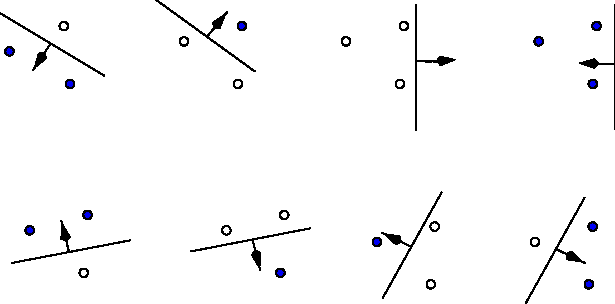
\includegraphics[width=0.7\textwidth]{Figs/PDF/vcdim_r2lines}
        \caption{All possible labellings of 3 points in $\mathbb{R}^2$ can be separated by a oriented line (2D hyperplane). This is not possible for all labellings of 4 points in $\mathbb{R}^2$ however, and thus the VC dimension of oriented hyperplanes in $\mathbb{R}^2$ is 3. From \citet{burges1998tutorial}.}
        \label{fig:vcdim_r2line}
    \end{figure}
    The information theoretic notion of capacity, that is the expressive power of a classification algorithm, gives important insights to the learning ability of a classification algorithm. Analysis is typically based on the Vapnik–Chervonenkis (VC) dimension~\citep{vapnik2015uniform} of the class of functions used as discriminators, \eg hyperplanes in the case of neural networks. Intuitively, for a discriminative classifier, the VC dimension measures the largest number of points that can be classified without error. In such a case, the set of points is said to be \emph{shattered} by the classifier. A good overview of VC-dimension is given by \citet{burges1998tutorial}.
    
    More formally, a classification model $f(\theta)$, parameterized by $\theta$ is said to \emph{shatter} a set of data points $(x_0, x_1, \ldots, x_h)$ if for for all possible labelings of the points, the classification model can perfectly learn the points. The Vapnik-Chervonenkis (VC) dimension is the largest number of (any) points that can be shattered by such a classifier. For a classifier of VC-dimension $h$, it is sufficient that there exists one set of $h$ points which can be shattered. It is important to note that in general a classifier with a VC-dimension of $h$ will not necessarily shatter every possible set of $h$ points. 
    %Note that, if the VC dimension is h, then there exists at least one set of h points that can be shattered, but it in general it will not be true that every set of h points can be shattered
    
    For example, in Fig.\ \ref{fig:vcdim_r2line}, the function class of oriented hyperplanes, \ie lines in 2D, can separate all possible labellings of 3 points in $\mathbb{R}^2$ -- oriented hyperplanes in $\mathbb{R}^2$ shatter 3 points. However, for 4 points, this is no longer true. It can be proven (see~\citet{burges1998tutorial}) that in general for $\mathbb{R}^n$, the set of oriented hyperplanes shatters any set of $n+1$ points.

    The VC dimension can give a measure of theoretical learning capacity of a classifier, however it can also be somewhat counter-intuitive. While models with large numbers of parameters usually will have a higher VC dimension, there are examples of small single parameter models with infinite VC dimension for more specific sets of points. For example, if we have a set of evenly spaced points in 2D, a simple sinusoidal curve with the appropriate phase can shatter any labeling of an infinite number of such points. However, in general such a classifier would be poor at classifying more general sets of points.
    
    In the case of neural networks, early work showed that the capacity of neural networks is quite large~\citep{hornik89a,baum1989size}.\todo{expand here! put some math}
    
    This however did not match empirical results. Later work showed that rather than capacity being based on solely the number of weights, instead the number of large weights was a better measure~\citep{bartlett1997}
    
    \todo{Include references to \citet{caruana2001overfitting, baum1989size, rethinking2016}}
	
    \subsection{Model Size}
	\begin{chapquote}{John Denker \etal, \textit{Large Automatic Learning, Complex Systems,1987}}
		``A general tabula rasa network is a fine subject for the abstract, formal studies, but one should not try to use it to solve practical problems. \ldots One should pre-program the network with all available information about the structure of the problem, especially information about the symmetry and topology of the data.''
	\end{chapquote}
	
	\begin{figure}[tb]
		\centering
		\begin{subfigure}[t]{0.49\textwidth}
			\resizebox{\linewidth}{!}{%% Creator: Matplotlib, PGF backend
%%
%% To include the figure in your LaTeX document, write
%%   \input{<filename>.pgf}
%%
%% Make sure the required packages are loaded in your preamble
%%   \usepackage{pgf}
%%
%% Figures using additional raster images can only be included by \input if
%% they are in the same directory as the main LaTeX file. For loading figures
%% from other directories you can use the `import` package
%%   \usepackage{import}
%% and then include the figures with
%%   \import{<path to file>}{<filename>.pgf}
%%
%% Matplotlib used the following preamble
%%   \usepackage[utf8x]{inputenc}
%%   \usepackage[T1]{fontenc}
%%
\begingroup%
\makeatletter%
\begin{pgfpicture}%
\pgfpathrectangle{\pgfpointorigin}{\pgfqpoint{4.296389in}{2.655314in}}%
\pgfusepath{use as bounding box, clip}%
\begin{pgfscope}%
\pgfsetbuttcap%
\pgfsetmiterjoin%
\definecolor{currentfill}{rgb}{1.000000,1.000000,1.000000}%
\pgfsetfillcolor{currentfill}%
\pgfsetlinewidth{0.000000pt}%
\definecolor{currentstroke}{rgb}{1.000000,1.000000,1.000000}%
\pgfsetstrokecolor{currentstroke}%
\pgfsetdash{}{0pt}%
\pgfpathmoveto{\pgfqpoint{0.000000in}{0.000000in}}%
\pgfpathlineto{\pgfqpoint{4.296389in}{0.000000in}}%
\pgfpathlineto{\pgfqpoint{4.296389in}{2.655314in}}%
\pgfpathlineto{\pgfqpoint{0.000000in}{2.655314in}}%
\pgfpathclose%
\pgfusepath{fill}%
\end{pgfscope}%
\begin{pgfscope}%
\pgfsetbuttcap%
\pgfsetmiterjoin%
\definecolor{currentfill}{rgb}{1.000000,1.000000,1.000000}%
\pgfsetfillcolor{currentfill}%
\pgfsetlinewidth{0.000000pt}%
\definecolor{currentstroke}{rgb}{0.000000,0.000000,0.000000}%
\pgfsetstrokecolor{currentstroke}%
\pgfsetstrokeopacity{0.000000}%
\pgfsetdash{}{0pt}%
\pgfpathmoveto{\pgfqpoint{0.548317in}{0.386884in}}%
\pgfpathlineto{\pgfqpoint{4.124652in}{0.386884in}}%
\pgfpathlineto{\pgfqpoint{4.124652in}{2.488647in}}%
\pgfpathlineto{\pgfqpoint{0.548317in}{2.488647in}}%
\pgfpathclose%
\pgfusepath{fill}%
\end{pgfscope}%
\begin{pgfscope}%
\pgfsetbuttcap%
\pgfsetroundjoin%
\definecolor{currentfill}{rgb}{0.150000,0.150000,0.150000}%
\pgfsetfillcolor{currentfill}%
\pgfsetlinewidth{1.003750pt}%
\definecolor{currentstroke}{rgb}{0.150000,0.150000,0.150000}%
\pgfsetstrokecolor{currentstroke}%
\pgfsetdash{}{0pt}%
\pgfsys@defobject{currentmarker}{\pgfqpoint{0.000000in}{-0.083333in}}{\pgfqpoint{0.000000in}{0.000000in}}{%
\pgfpathmoveto{\pgfqpoint{0.000000in}{0.000000in}}%
\pgfpathlineto{\pgfqpoint{0.000000in}{-0.083333in}}%
\pgfusepath{stroke,fill}%
}%
\begin{pgfscope}%
\pgfsys@transformshift{0.548317in}{0.386884in}%
\pgfsys@useobject{currentmarker}{}%
\end{pgfscope}%
\end{pgfscope}%
\begin{pgfscope}%
\definecolor{textcolor}{rgb}{0.150000,0.150000,0.150000}%
\pgfsetstrokecolor{textcolor}%
\pgfsetfillcolor{textcolor}%
\pgftext[x=0.548317in,y=0.206329in,,top]{\color{textcolor}\sffamily\fontsize{10.000000}{12.000000}\selectfont \(\displaystyle 0.0\)}%
\end{pgfscope}%
\begin{pgfscope}%
\pgfsetbuttcap%
\pgfsetroundjoin%
\definecolor{currentfill}{rgb}{0.150000,0.150000,0.150000}%
\pgfsetfillcolor{currentfill}%
\pgfsetlinewidth{1.003750pt}%
\definecolor{currentstroke}{rgb}{0.150000,0.150000,0.150000}%
\pgfsetstrokecolor{currentstroke}%
\pgfsetdash{}{0pt}%
\pgfsys@defobject{currentmarker}{\pgfqpoint{0.000000in}{-0.083333in}}{\pgfqpoint{0.000000in}{0.000000in}}{%
\pgfpathmoveto{\pgfqpoint{0.000000in}{0.000000in}}%
\pgfpathlineto{\pgfqpoint{0.000000in}{-0.083333in}}%
\pgfusepath{stroke,fill}%
}%
\begin{pgfscope}%
\pgfsys@transformshift{1.263584in}{0.386884in}%
\pgfsys@useobject{currentmarker}{}%
\end{pgfscope}%
\end{pgfscope}%
\begin{pgfscope}%
\definecolor{textcolor}{rgb}{0.150000,0.150000,0.150000}%
\pgfsetstrokecolor{textcolor}%
\pgfsetfillcolor{textcolor}%
\pgftext[x=1.263584in,y=0.206329in,,top]{\color{textcolor}\sffamily\fontsize{10.000000}{12.000000}\selectfont \(\displaystyle 0.2\)}%
\end{pgfscope}%
\begin{pgfscope}%
\pgfsetbuttcap%
\pgfsetroundjoin%
\definecolor{currentfill}{rgb}{0.150000,0.150000,0.150000}%
\pgfsetfillcolor{currentfill}%
\pgfsetlinewidth{1.003750pt}%
\definecolor{currentstroke}{rgb}{0.150000,0.150000,0.150000}%
\pgfsetstrokecolor{currentstroke}%
\pgfsetdash{}{0pt}%
\pgfsys@defobject{currentmarker}{\pgfqpoint{0.000000in}{-0.083333in}}{\pgfqpoint{0.000000in}{0.000000in}}{%
\pgfpathmoveto{\pgfqpoint{0.000000in}{0.000000in}}%
\pgfpathlineto{\pgfqpoint{0.000000in}{-0.083333in}}%
\pgfusepath{stroke,fill}%
}%
\begin{pgfscope}%
\pgfsys@transformshift{1.978851in}{0.386884in}%
\pgfsys@useobject{currentmarker}{}%
\end{pgfscope}%
\end{pgfscope}%
\begin{pgfscope}%
\definecolor{textcolor}{rgb}{0.150000,0.150000,0.150000}%
\pgfsetstrokecolor{textcolor}%
\pgfsetfillcolor{textcolor}%
\pgftext[x=1.978851in,y=0.206329in,,top]{\color{textcolor}\sffamily\fontsize{10.000000}{12.000000}\selectfont \(\displaystyle 0.4\)}%
\end{pgfscope}%
\begin{pgfscope}%
\pgfsetbuttcap%
\pgfsetroundjoin%
\definecolor{currentfill}{rgb}{0.150000,0.150000,0.150000}%
\pgfsetfillcolor{currentfill}%
\pgfsetlinewidth{1.003750pt}%
\definecolor{currentstroke}{rgb}{0.150000,0.150000,0.150000}%
\pgfsetstrokecolor{currentstroke}%
\pgfsetdash{}{0pt}%
\pgfsys@defobject{currentmarker}{\pgfqpoint{0.000000in}{-0.083333in}}{\pgfqpoint{0.000000in}{0.000000in}}{%
\pgfpathmoveto{\pgfqpoint{0.000000in}{0.000000in}}%
\pgfpathlineto{\pgfqpoint{0.000000in}{-0.083333in}}%
\pgfusepath{stroke,fill}%
}%
\begin{pgfscope}%
\pgfsys@transformshift{2.694118in}{0.386884in}%
\pgfsys@useobject{currentmarker}{}%
\end{pgfscope}%
\end{pgfscope}%
\begin{pgfscope}%
\definecolor{textcolor}{rgb}{0.150000,0.150000,0.150000}%
\pgfsetstrokecolor{textcolor}%
\pgfsetfillcolor{textcolor}%
\pgftext[x=2.694118in,y=0.206329in,,top]{\color{textcolor}\sffamily\fontsize{10.000000}{12.000000}\selectfont \(\displaystyle 0.6\)}%
\end{pgfscope}%
\begin{pgfscope}%
\pgfsetbuttcap%
\pgfsetroundjoin%
\definecolor{currentfill}{rgb}{0.150000,0.150000,0.150000}%
\pgfsetfillcolor{currentfill}%
\pgfsetlinewidth{1.003750pt}%
\definecolor{currentstroke}{rgb}{0.150000,0.150000,0.150000}%
\pgfsetstrokecolor{currentstroke}%
\pgfsetdash{}{0pt}%
\pgfsys@defobject{currentmarker}{\pgfqpoint{0.000000in}{-0.083333in}}{\pgfqpoint{0.000000in}{0.000000in}}{%
\pgfpathmoveto{\pgfqpoint{0.000000in}{0.000000in}}%
\pgfpathlineto{\pgfqpoint{0.000000in}{-0.083333in}}%
\pgfusepath{stroke,fill}%
}%
\begin{pgfscope}%
\pgfsys@transformshift{3.409385in}{0.386884in}%
\pgfsys@useobject{currentmarker}{}%
\end{pgfscope}%
\end{pgfscope}%
\begin{pgfscope}%
\definecolor{textcolor}{rgb}{0.150000,0.150000,0.150000}%
\pgfsetstrokecolor{textcolor}%
\pgfsetfillcolor{textcolor}%
\pgftext[x=3.409385in,y=0.206329in,,top]{\color{textcolor}\sffamily\fontsize{10.000000}{12.000000}\selectfont \(\displaystyle 0.8\)}%
\end{pgfscope}%
\begin{pgfscope}%
\pgfsetbuttcap%
\pgfsetroundjoin%
\definecolor{currentfill}{rgb}{0.150000,0.150000,0.150000}%
\pgfsetfillcolor{currentfill}%
\pgfsetlinewidth{1.003750pt}%
\definecolor{currentstroke}{rgb}{0.150000,0.150000,0.150000}%
\pgfsetstrokecolor{currentstroke}%
\pgfsetdash{}{0pt}%
\pgfsys@defobject{currentmarker}{\pgfqpoint{0.000000in}{-0.083333in}}{\pgfqpoint{0.000000in}{0.000000in}}{%
\pgfpathmoveto{\pgfqpoint{0.000000in}{0.000000in}}%
\pgfpathlineto{\pgfqpoint{0.000000in}{-0.083333in}}%
\pgfusepath{stroke,fill}%
}%
\begin{pgfscope}%
\pgfsys@transformshift{4.124652in}{0.386884in}%
\pgfsys@useobject{currentmarker}{}%
\end{pgfscope}%
\end{pgfscope}%
\begin{pgfscope}%
\definecolor{textcolor}{rgb}{0.150000,0.150000,0.150000}%
\pgfsetstrokecolor{textcolor}%
\pgfsetfillcolor{textcolor}%
\pgftext[x=4.124652in,y=0.206329in,,top]{\color{textcolor}\sffamily\fontsize{10.000000}{12.000000}\selectfont \(\displaystyle 1.0\)}%
\end{pgfscope}%
\begin{pgfscope}%
\pgfsetbuttcap%
\pgfsetroundjoin%
\definecolor{currentfill}{rgb}{0.150000,0.150000,0.150000}%
\pgfsetfillcolor{currentfill}%
\pgfsetlinewidth{1.003750pt}%
\definecolor{currentstroke}{rgb}{0.150000,0.150000,0.150000}%
\pgfsetstrokecolor{currentstroke}%
\pgfsetdash{}{0pt}%
\pgfsys@defobject{currentmarker}{\pgfqpoint{-0.083333in}{0.000000in}}{\pgfqpoint{0.000000in}{0.000000in}}{%
\pgfpathmoveto{\pgfqpoint{0.000000in}{0.000000in}}%
\pgfpathlineto{\pgfqpoint{-0.083333in}{0.000000in}}%
\pgfusepath{stroke,fill}%
}%
\begin{pgfscope}%
\pgfsys@transformshift{0.548317in}{0.386884in}%
\pgfsys@useobject{currentmarker}{}%
\end{pgfscope}%
\end{pgfscope}%
\begin{pgfscope}%
\definecolor{textcolor}{rgb}{0.150000,0.150000,0.150000}%
\pgfsetstrokecolor{textcolor}%
\pgfsetfillcolor{textcolor}%
\pgftext[x=0.082267in,y=0.336742in,left,base]{\color{textcolor}\sffamily\fontsize{10.000000}{12.000000}\selectfont \(\displaystyle -1.0\)}%
\end{pgfscope}%
\begin{pgfscope}%
\pgfsetbuttcap%
\pgfsetroundjoin%
\definecolor{currentfill}{rgb}{0.150000,0.150000,0.150000}%
\pgfsetfillcolor{currentfill}%
\pgfsetlinewidth{1.003750pt}%
\definecolor{currentstroke}{rgb}{0.150000,0.150000,0.150000}%
\pgfsetstrokecolor{currentstroke}%
\pgfsetdash{}{0pt}%
\pgfsys@defobject{currentmarker}{\pgfqpoint{-0.083333in}{0.000000in}}{\pgfqpoint{0.000000in}{0.000000in}}{%
\pgfpathmoveto{\pgfqpoint{0.000000in}{0.000000in}}%
\pgfpathlineto{\pgfqpoint{-0.083333in}{0.000000in}}%
\pgfusepath{stroke,fill}%
}%
\begin{pgfscope}%
\pgfsys@transformshift{0.548317in}{0.912325in}%
\pgfsys@useobject{currentmarker}{}%
\end{pgfscope}%
\end{pgfscope}%
\begin{pgfscope}%
\definecolor{textcolor}{rgb}{0.150000,0.150000,0.150000}%
\pgfsetstrokecolor{textcolor}%
\pgfsetfillcolor{textcolor}%
\pgftext[x=0.082267in,y=0.862183in,left,base]{\color{textcolor}\sffamily\fontsize{10.000000}{12.000000}\selectfont \(\displaystyle -0.5\)}%
\end{pgfscope}%
\begin{pgfscope}%
\pgfsetbuttcap%
\pgfsetroundjoin%
\definecolor{currentfill}{rgb}{0.150000,0.150000,0.150000}%
\pgfsetfillcolor{currentfill}%
\pgfsetlinewidth{1.003750pt}%
\definecolor{currentstroke}{rgb}{0.150000,0.150000,0.150000}%
\pgfsetstrokecolor{currentstroke}%
\pgfsetdash{}{0pt}%
\pgfsys@defobject{currentmarker}{\pgfqpoint{-0.083333in}{0.000000in}}{\pgfqpoint{0.000000in}{0.000000in}}{%
\pgfpathmoveto{\pgfqpoint{0.000000in}{0.000000in}}%
\pgfpathlineto{\pgfqpoint{-0.083333in}{0.000000in}}%
\pgfusepath{stroke,fill}%
}%
\begin{pgfscope}%
\pgfsys@transformshift{0.548317in}{1.437766in}%
\pgfsys@useobject{currentmarker}{}%
\end{pgfscope}%
\end{pgfscope}%
\begin{pgfscope}%
\definecolor{textcolor}{rgb}{0.150000,0.150000,0.150000}%
\pgfsetstrokecolor{textcolor}%
\pgfsetfillcolor{textcolor}%
\pgftext[x=0.190292in,y=1.387624in,left,base]{\color{textcolor}\sffamily\fontsize{10.000000}{12.000000}\selectfont \(\displaystyle 0.0\)}%
\end{pgfscope}%
\begin{pgfscope}%
\pgfsetbuttcap%
\pgfsetroundjoin%
\definecolor{currentfill}{rgb}{0.150000,0.150000,0.150000}%
\pgfsetfillcolor{currentfill}%
\pgfsetlinewidth{1.003750pt}%
\definecolor{currentstroke}{rgb}{0.150000,0.150000,0.150000}%
\pgfsetstrokecolor{currentstroke}%
\pgfsetdash{}{0pt}%
\pgfsys@defobject{currentmarker}{\pgfqpoint{-0.083333in}{0.000000in}}{\pgfqpoint{0.000000in}{0.000000in}}{%
\pgfpathmoveto{\pgfqpoint{0.000000in}{0.000000in}}%
\pgfpathlineto{\pgfqpoint{-0.083333in}{0.000000in}}%
\pgfusepath{stroke,fill}%
}%
\begin{pgfscope}%
\pgfsys@transformshift{0.548317in}{1.963207in}%
\pgfsys@useobject{currentmarker}{}%
\end{pgfscope}%
\end{pgfscope}%
\begin{pgfscope}%
\definecolor{textcolor}{rgb}{0.150000,0.150000,0.150000}%
\pgfsetstrokecolor{textcolor}%
\pgfsetfillcolor{textcolor}%
\pgftext[x=0.190292in,y=1.913065in,left,base]{\color{textcolor}\sffamily\fontsize{10.000000}{12.000000}\selectfont \(\displaystyle 0.5\)}%
\end{pgfscope}%
\begin{pgfscope}%
\pgfsetbuttcap%
\pgfsetroundjoin%
\definecolor{currentfill}{rgb}{0.150000,0.150000,0.150000}%
\pgfsetfillcolor{currentfill}%
\pgfsetlinewidth{1.003750pt}%
\definecolor{currentstroke}{rgb}{0.150000,0.150000,0.150000}%
\pgfsetstrokecolor{currentstroke}%
\pgfsetdash{}{0pt}%
\pgfsys@defobject{currentmarker}{\pgfqpoint{-0.083333in}{0.000000in}}{\pgfqpoint{0.000000in}{0.000000in}}{%
\pgfpathmoveto{\pgfqpoint{0.000000in}{0.000000in}}%
\pgfpathlineto{\pgfqpoint{-0.083333in}{0.000000in}}%
\pgfusepath{stroke,fill}%
}%
\begin{pgfscope}%
\pgfsys@transformshift{0.548317in}{2.488647in}%
\pgfsys@useobject{currentmarker}{}%
\end{pgfscope}%
\end{pgfscope}%
\begin{pgfscope}%
\definecolor{textcolor}{rgb}{0.150000,0.150000,0.150000}%
\pgfsetstrokecolor{textcolor}%
\pgfsetfillcolor{textcolor}%
\pgftext[x=0.190292in,y=2.438505in,left,base]{\color{textcolor}\sffamily\fontsize{10.000000}{12.000000}\selectfont \(\displaystyle 1.0\)}%
\end{pgfscope}%
\begin{pgfscope}%
\pgfpathrectangle{\pgfqpoint{0.548317in}{0.386884in}}{\pgfqpoint{3.576335in}{2.101763in}} %
\pgfusepath{clip}%
\pgfsetbuttcap%
\pgfsetroundjoin%
\definecolor{currentfill}{rgb}{0.400000,0.760784,0.647059}%
\pgfsetfillcolor{currentfill}%
\pgfsetlinewidth{0.000000pt}%
\definecolor{currentstroke}{rgb}{0.400000,0.760784,0.647059}%
\pgfsetstrokecolor{currentstroke}%
\pgfsetdash{}{0pt}%
\pgfsys@defobject{currentmarker}{\pgfqpoint{-0.048611in}{-0.048611in}}{\pgfqpoint{0.048611in}{0.048611in}}{%
\pgfpathmoveto{\pgfqpoint{0.000000in}{-0.048611in}}%
\pgfpathcurveto{\pgfqpoint{0.012892in}{-0.048611in}}{\pgfqpoint{0.025257in}{-0.043489in}}{\pgfqpoint{0.034373in}{-0.034373in}}%
\pgfpathcurveto{\pgfqpoint{0.043489in}{-0.025257in}}{\pgfqpoint{0.048611in}{-0.012892in}}{\pgfqpoint{0.048611in}{0.000000in}}%
\pgfpathcurveto{\pgfqpoint{0.048611in}{0.012892in}}{\pgfqpoint{0.043489in}{0.025257in}}{\pgfqpoint{0.034373in}{0.034373in}}%
\pgfpathcurveto{\pgfqpoint{0.025257in}{0.043489in}}{\pgfqpoint{0.012892in}{0.048611in}}{\pgfqpoint{0.000000in}{0.048611in}}%
\pgfpathcurveto{\pgfqpoint{-0.012892in}{0.048611in}}{\pgfqpoint{-0.025257in}{0.043489in}}{\pgfqpoint{-0.034373in}{0.034373in}}%
\pgfpathcurveto{\pgfqpoint{-0.043489in}{0.025257in}}{\pgfqpoint{-0.048611in}{0.012892in}}{\pgfqpoint{-0.048611in}{0.000000in}}%
\pgfpathcurveto{\pgfqpoint{-0.048611in}{-0.012892in}}{\pgfqpoint{-0.043489in}{-0.025257in}}{\pgfqpoint{-0.034373in}{-0.034373in}}%
\pgfpathcurveto{\pgfqpoint{-0.025257in}{-0.043489in}}{\pgfqpoint{-0.012892in}{-0.048611in}}{\pgfqpoint{0.000000in}{-0.048611in}}%
\pgfpathclose%
\pgfusepath{fill}%
}%
\begin{pgfscope}%
\pgfsys@transformshift{2.260811in}{0.754316in}%
\pgfsys@useobject{currentmarker}{}%
\end{pgfscope}%
\begin{pgfscope}%
\pgfsys@transformshift{2.611975in}{0.899184in}%
\pgfsys@useobject{currentmarker}{}%
\end{pgfscope}%
\begin{pgfscope}%
\pgfsys@transformshift{3.012052in}{1.144101in}%
\pgfsys@useobject{currentmarker}{}%
\end{pgfscope}%
\end{pgfscope}%
\begin{pgfscope}%
\pgfpathrectangle{\pgfqpoint{0.548317in}{0.386884in}}{\pgfqpoint{3.576335in}{2.101763in}} %
\pgfusepath{clip}%
\pgfsetbuttcap%
\pgfsetroundjoin%
\pgfsetlinewidth{1.756562pt}%
\definecolor{currentstroke}{rgb}{0.988235,0.552941,0.384314}%
\pgfsetstrokecolor{currentstroke}%
\pgfsetdash{{5.600000pt}{2.400000pt}}{0.000000pt}%
\pgfpathmoveto{\pgfqpoint{0.534428in}{0.382588in}}%
\pgfpathlineto{\pgfqpoint{0.584442in}{0.397288in}}%
\pgfpathlineto{\pgfqpoint{0.656691in}{0.416887in}}%
\pgfpathlineto{\pgfqpoint{0.728940in}{0.435004in}}%
\pgfpathlineto{\pgfqpoint{0.801189in}{0.451796in}}%
\pgfpathlineto{\pgfqpoint{0.873438in}{0.467418in}}%
\pgfpathlineto{\pgfqpoint{0.945688in}{0.482026in}}%
\pgfpathlineto{\pgfqpoint{1.017937in}{0.495776in}}%
\pgfpathlineto{\pgfqpoint{1.090186in}{0.508825in}}%
\pgfpathlineto{\pgfqpoint{1.162435in}{0.521328in}}%
\pgfpathlineto{\pgfqpoint{1.234684in}{0.533440in}}%
\pgfpathlineto{\pgfqpoint{1.306933in}{0.545319in}}%
\pgfpathlineto{\pgfqpoint{1.379183in}{0.557120in}}%
\pgfpathlineto{\pgfqpoint{1.451432in}{0.568999in}}%
\pgfpathlineto{\pgfqpoint{1.523681in}{0.581112in}}%
\pgfpathlineto{\pgfqpoint{1.595930in}{0.593615in}}%
\pgfpathlineto{\pgfqpoint{1.668179in}{0.606663in}}%
\pgfpathlineto{\pgfqpoint{1.740429in}{0.620414in}}%
\pgfpathlineto{\pgfqpoint{1.812678in}{0.635022in}}%
\pgfpathlineto{\pgfqpoint{1.884927in}{0.650644in}}%
\pgfpathlineto{\pgfqpoint{1.957176in}{0.667435in}}%
\pgfpathlineto{\pgfqpoint{2.029425in}{0.685553in}}%
\pgfpathlineto{\pgfqpoint{2.101675in}{0.705151in}}%
\pgfpathlineto{\pgfqpoint{2.173924in}{0.726388in}}%
\pgfpathlineto{\pgfqpoint{2.246173in}{0.749418in}}%
\pgfpathlineto{\pgfqpoint{2.318422in}{0.774397in}}%
\pgfpathlineto{\pgfqpoint{2.390671in}{0.801482in}}%
\pgfpathlineto{\pgfqpoint{2.462921in}{0.830828in}}%
\pgfpathlineto{\pgfqpoint{2.535170in}{0.862592in}}%
\pgfpathlineto{\pgfqpoint{2.607419in}{0.896929in}}%
\pgfpathlineto{\pgfqpoint{2.679668in}{0.933995in}}%
\pgfpathlineto{\pgfqpoint{2.751917in}{0.973947in}}%
\pgfpathlineto{\pgfqpoint{2.824166in}{1.016940in}}%
\pgfpathlineto{\pgfqpoint{2.896416in}{1.063129in}}%
\pgfpathlineto{\pgfqpoint{2.968665in}{1.112672in}}%
\pgfpathlineto{\pgfqpoint{3.040914in}{1.165725in}}%
\pgfpathlineto{\pgfqpoint{3.113163in}{1.222442in}}%
\pgfpathlineto{\pgfqpoint{3.185412in}{1.282980in}}%
\pgfpathlineto{\pgfqpoint{3.257662in}{1.347495in}}%
\pgfpathlineto{\pgfqpoint{3.329911in}{1.416143in}}%
\pgfpathlineto{\pgfqpoint{3.402160in}{1.489080in}}%
\pgfpathlineto{\pgfqpoint{3.474409in}{1.566461in}}%
\pgfpathlineto{\pgfqpoint{3.546658in}{1.648444in}}%
\pgfpathlineto{\pgfqpoint{3.618908in}{1.735183in}}%
\pgfpathlineto{\pgfqpoint{3.691157in}{1.826835in}}%
\pgfpathlineto{\pgfqpoint{3.763406in}{1.923556in}}%
\pgfpathlineto{\pgfqpoint{3.835655in}{2.025501in}}%
\pgfpathlineto{\pgfqpoint{3.907904in}{2.132827in}}%
\pgfpathlineto{\pgfqpoint{3.980154in}{2.245689in}}%
\pgfpathlineto{\pgfqpoint{4.052403in}{2.364244in}}%
\pgfpathlineto{\pgfqpoint{4.124652in}{2.488647in}}%
\pgfusepath{stroke}%
\end{pgfscope}%
\begin{pgfscope}%
\pgfpathrectangle{\pgfqpoint{0.548317in}{0.386884in}}{\pgfqpoint{3.576335in}{2.101763in}} %
\pgfusepath{clip}%
\pgfsetroundcap%
\pgfsetroundjoin%
\pgfsetlinewidth{1.756562pt}%
\definecolor{currentstroke}{rgb}{0.552941,0.627451,0.796078}%
\pgfsetstrokecolor{currentstroke}%
\pgfsetdash{}{0pt}%
\pgfpathmoveto{\pgfqpoint{0.534428in}{0.664235in}}%
\pgfpathlineto{\pgfqpoint{0.584442in}{0.658600in}}%
\pgfpathlineto{\pgfqpoint{0.656691in}{0.650850in}}%
\pgfpathlineto{\pgfqpoint{0.728940in}{0.643574in}}%
\pgfpathlineto{\pgfqpoint{0.801189in}{0.636856in}}%
\pgfpathlineto{\pgfqpoint{0.873438in}{0.630780in}}%
\pgfpathlineto{\pgfqpoint{0.945688in}{0.625432in}}%
\pgfpathlineto{\pgfqpoint{1.017937in}{0.620894in}}%
\pgfpathlineto{\pgfqpoint{1.090186in}{0.617252in}}%
\pgfpathlineto{\pgfqpoint{1.162435in}{0.614590in}}%
\pgfpathlineto{\pgfqpoint{1.234684in}{0.612992in}}%
\pgfpathlineto{\pgfqpoint{1.306933in}{0.612542in}}%
\pgfpathlineto{\pgfqpoint{1.379183in}{0.613325in}}%
\pgfpathlineto{\pgfqpoint{1.451432in}{0.615424in}}%
\pgfpathlineto{\pgfqpoint{1.523681in}{0.618925in}}%
\pgfpathlineto{\pgfqpoint{1.595930in}{0.623912in}}%
\pgfpathlineto{\pgfqpoint{1.668179in}{0.630468in}}%
\pgfpathlineto{\pgfqpoint{1.740429in}{0.638678in}}%
\pgfpathlineto{\pgfqpoint{1.812678in}{0.648627in}}%
\pgfpathlineto{\pgfqpoint{1.884927in}{0.660399in}}%
\pgfpathlineto{\pgfqpoint{1.957176in}{0.674077in}}%
\pgfpathlineto{\pgfqpoint{2.029425in}{0.689747in}}%
\pgfpathlineto{\pgfqpoint{2.101675in}{0.707493in}}%
\pgfpathlineto{\pgfqpoint{2.173924in}{0.727398in}}%
\pgfpathlineto{\pgfqpoint{2.246173in}{0.749548in}}%
\pgfpathlineto{\pgfqpoint{2.318422in}{0.774026in}}%
\pgfpathlineto{\pgfqpoint{2.390671in}{0.800917in}}%
\pgfpathlineto{\pgfqpoint{2.462921in}{0.830305in}}%
\pgfpathlineto{\pgfqpoint{2.535170in}{0.862274in}}%
\pgfpathlineto{\pgfqpoint{2.607419in}{0.896909in}}%
\pgfpathlineto{\pgfqpoint{2.679668in}{0.934294in}}%
\pgfpathlineto{\pgfqpoint{2.751917in}{0.974513in}}%
\pgfpathlineto{\pgfqpoint{2.824166in}{1.017651in}}%
\pgfpathlineto{\pgfqpoint{2.896416in}{1.063792in}}%
\pgfpathlineto{\pgfqpoint{2.968665in}{1.113019in}}%
\pgfpathlineto{\pgfqpoint{3.040914in}{1.165419in}}%
\pgfpathlineto{\pgfqpoint{3.113163in}{1.221074in}}%
\pgfpathlineto{\pgfqpoint{3.185412in}{1.280069in}}%
\pgfpathlineto{\pgfqpoint{3.257662in}{1.342488in}}%
\pgfpathlineto{\pgfqpoint{3.329911in}{1.408416in}}%
\pgfpathlineto{\pgfqpoint{3.402160in}{1.477937in}}%
\pgfpathlineto{\pgfqpoint{3.474409in}{1.551136in}}%
\pgfpathlineto{\pgfqpoint{3.546658in}{1.628095in}}%
\pgfpathlineto{\pgfqpoint{3.618908in}{1.708901in}}%
\pgfpathlineto{\pgfqpoint{3.691157in}{1.793637in}}%
\pgfpathlineto{\pgfqpoint{3.763406in}{1.882387in}}%
\pgfpathlineto{\pgfqpoint{3.835655in}{1.975236in}}%
\pgfpathlineto{\pgfqpoint{3.907904in}{2.072268in}}%
\pgfpathlineto{\pgfqpoint{3.980154in}{2.173567in}}%
\pgfpathlineto{\pgfqpoint{4.052403in}{2.279218in}}%
\pgfpathlineto{\pgfqpoint{4.124652in}{2.389305in}}%
\pgfusepath{stroke}%
\end{pgfscope}%
\begin{pgfscope}%
\pgfsetrectcap%
\pgfsetmiterjoin%
\pgfsetlinewidth{1.254687pt}%
\definecolor{currentstroke}{rgb}{0.150000,0.150000,0.150000}%
\pgfsetstrokecolor{currentstroke}%
\pgfsetdash{}{0pt}%
\pgfpathmoveto{\pgfqpoint{0.548317in}{0.386884in}}%
\pgfpathlineto{\pgfqpoint{0.548317in}{2.488647in}}%
\pgfusepath{stroke}%
\end{pgfscope}%
\begin{pgfscope}%
\pgfsetrectcap%
\pgfsetmiterjoin%
\pgfsetlinewidth{1.254687pt}%
\definecolor{currentstroke}{rgb}{0.150000,0.150000,0.150000}%
\pgfsetstrokecolor{currentstroke}%
\pgfsetdash{}{0pt}%
\pgfpathmoveto{\pgfqpoint{0.548317in}{0.386884in}}%
\pgfpathlineto{\pgfqpoint{4.124652in}{0.386884in}}%
\pgfusepath{stroke}%
\end{pgfscope}%
\begin{pgfscope}%
\pgfsetbuttcap%
\pgfsetroundjoin%
\definecolor{currentfill}{rgb}{0.400000,0.760784,0.647059}%
\pgfsetfillcolor{currentfill}%
\pgfsetlinewidth{0.000000pt}%
\definecolor{currentstroke}{rgb}{0.400000,0.760784,0.647059}%
\pgfsetstrokecolor{currentstroke}%
\pgfsetdash{}{0pt}%
\pgfsys@defobject{currentmarker}{\pgfqpoint{-0.048611in}{-0.048611in}}{\pgfqpoint{0.048611in}{0.048611in}}{%
\pgfpathmoveto{\pgfqpoint{0.000000in}{-0.048611in}}%
\pgfpathcurveto{\pgfqpoint{0.012892in}{-0.048611in}}{\pgfqpoint{0.025257in}{-0.043489in}}{\pgfqpoint{0.034373in}{-0.034373in}}%
\pgfpathcurveto{\pgfqpoint{0.043489in}{-0.025257in}}{\pgfqpoint{0.048611in}{-0.012892in}}{\pgfqpoint{0.048611in}{0.000000in}}%
\pgfpathcurveto{\pgfqpoint{0.048611in}{0.012892in}}{\pgfqpoint{0.043489in}{0.025257in}}{\pgfqpoint{0.034373in}{0.034373in}}%
\pgfpathcurveto{\pgfqpoint{0.025257in}{0.043489in}}{\pgfqpoint{0.012892in}{0.048611in}}{\pgfqpoint{0.000000in}{0.048611in}}%
\pgfpathcurveto{\pgfqpoint{-0.012892in}{0.048611in}}{\pgfqpoint{-0.025257in}{0.043489in}}{\pgfqpoint{-0.034373in}{0.034373in}}%
\pgfpathcurveto{\pgfqpoint{-0.043489in}{0.025257in}}{\pgfqpoint{-0.048611in}{0.012892in}}{\pgfqpoint{-0.048611in}{0.000000in}}%
\pgfpathcurveto{\pgfqpoint{-0.048611in}{-0.012892in}}{\pgfqpoint{-0.043489in}{-0.025257in}}{\pgfqpoint{-0.034373in}{-0.034373in}}%
\pgfpathcurveto{\pgfqpoint{-0.025257in}{-0.043489in}}{\pgfqpoint{-0.012892in}{-0.048611in}}{\pgfqpoint{0.000000in}{-0.048611in}}%
\pgfpathclose%
\pgfusepath{fill}%
}%
\begin{pgfscope}%
\pgfsys@transformshift{0.812206in}{2.311974in}%
\pgfsys@useobject{currentmarker}{}%
\end{pgfscope}%
\end{pgfscope}%
\begin{pgfscope}%
\definecolor{textcolor}{rgb}{0.150000,0.150000,0.150000}%
\pgfsetstrokecolor{textcolor}%
\pgfsetfillcolor{textcolor}%
\pgftext[x=1.062206in,y=2.263363in,left,base]{\color{textcolor}\sffamily\fontsize{10.000000}{12.000000}\selectfont samples}%
\end{pgfscope}%
\begin{pgfscope}%
\pgfsetbuttcap%
\pgfsetroundjoin%
\pgfsetlinewidth{1.756562pt}%
\definecolor{currentstroke}{rgb}{0.988235,0.552941,0.384314}%
\pgfsetstrokecolor{currentstroke}%
\pgfsetdash{{5.600000pt}{2.400000pt}}{0.000000pt}%
\pgfpathmoveto{\pgfqpoint{0.673317in}{2.115246in}}%
\pgfpathlineto{\pgfqpoint{0.951095in}{2.115246in}}%
\pgfusepath{stroke}%
\end{pgfscope}%
\begin{pgfscope}%
\definecolor{textcolor}{rgb}{0.150000,0.150000,0.150000}%
\pgfsetstrokecolor{textcolor}%
\pgfsetfillcolor{textcolor}%
\pgftext[x=1.062206in,y=2.066635in,left,base]{\color{textcolor}\sffamily\fontsize{10.000000}{12.000000}\selectfont function}%
\end{pgfscope}%
\begin{pgfscope}%
\pgfsetroundcap%
\pgfsetroundjoin%
\pgfsetlinewidth{1.756562pt}%
\definecolor{currentstroke}{rgb}{0.552941,0.627451,0.796078}%
\pgfsetstrokecolor{currentstroke}%
\pgfsetdash{}{0pt}%
\pgfpathmoveto{\pgfqpoint{0.673317in}{1.918518in}}%
\pgfpathlineto{\pgfqpoint{0.951095in}{1.918518in}}%
\pgfusepath{stroke}%
\end{pgfscope}%
\begin{pgfscope}%
\definecolor{textcolor}{rgb}{0.150000,0.150000,0.150000}%
\pgfsetstrokecolor{textcolor}%
\pgfsetfillcolor{textcolor}%
\pgftext[x=1.062206in,y=1.869907in,left,base]{\color{textcolor}\sffamily\fontsize{10.000000}{12.000000}\selectfont 3rd order fit}%
\end{pgfscope}%
\end{pgfpicture}%
\makeatother%
\endgroup%
}
			\caption{\engordnumber{3}-order polynomial fitting 3 points}
			\label{fig:polyfit3rd}
		\end{subfigure}
		~
		\begin{subfigure}[t]{0.49\textwidth}
			\resizebox{\linewidth}{!}{%% Creator: Matplotlib, PGF backend
%%
%% To include the figure in your LaTeX document, write
%%   \input{<filename>.pgf}
%%
%% Make sure the required packages are loaded in your preamble
%%   \usepackage{pgf}
%%
%% Figures using additional raster images can only be included by \input if
%% they are in the same directory as the main LaTeX file. For loading figures
%% from other directories you can use the `import` package
%%   \usepackage{import}
%% and then include the figures with
%%   \import{<path to file>}{<filename>.pgf}
%%
%% Matplotlib used the following preamble
%%   \usepackage[utf8x]{inputenc}
%%   \usepackage[T1]{fontenc}
%%
\begingroup%
\makeatletter%
\begin{pgfpicture}%
\pgfpathrectangle{\pgfpointorigin}{\pgfqpoint{4.296389in}{2.655314in}}%
\pgfusepath{use as bounding box, clip}%
\begin{pgfscope}%
\pgfsetbuttcap%
\pgfsetmiterjoin%
\definecolor{currentfill}{rgb}{1.000000,1.000000,1.000000}%
\pgfsetfillcolor{currentfill}%
\pgfsetlinewidth{0.000000pt}%
\definecolor{currentstroke}{rgb}{1.000000,1.000000,1.000000}%
\pgfsetstrokecolor{currentstroke}%
\pgfsetdash{}{0pt}%
\pgfpathmoveto{\pgfqpoint{0.000000in}{0.000000in}}%
\pgfpathlineto{\pgfqpoint{4.296389in}{0.000000in}}%
\pgfpathlineto{\pgfqpoint{4.296389in}{2.655314in}}%
\pgfpathlineto{\pgfqpoint{0.000000in}{2.655314in}}%
\pgfpathclose%
\pgfusepath{fill}%
\end{pgfscope}%
\begin{pgfscope}%
\pgfsetbuttcap%
\pgfsetmiterjoin%
\definecolor{currentfill}{rgb}{1.000000,1.000000,1.000000}%
\pgfsetfillcolor{currentfill}%
\pgfsetlinewidth{0.000000pt}%
\definecolor{currentstroke}{rgb}{0.000000,0.000000,0.000000}%
\pgfsetstrokecolor{currentstroke}%
\pgfsetstrokeopacity{0.000000}%
\pgfsetdash{}{0pt}%
\pgfpathmoveto{\pgfqpoint{0.548317in}{0.386884in}}%
\pgfpathlineto{\pgfqpoint{4.124652in}{0.386884in}}%
\pgfpathlineto{\pgfqpoint{4.124652in}{2.488647in}}%
\pgfpathlineto{\pgfqpoint{0.548317in}{2.488647in}}%
\pgfpathclose%
\pgfusepath{fill}%
\end{pgfscope}%
\begin{pgfscope}%
\pgfsetbuttcap%
\pgfsetroundjoin%
\definecolor{currentfill}{rgb}{0.150000,0.150000,0.150000}%
\pgfsetfillcolor{currentfill}%
\pgfsetlinewidth{1.003750pt}%
\definecolor{currentstroke}{rgb}{0.150000,0.150000,0.150000}%
\pgfsetstrokecolor{currentstroke}%
\pgfsetdash{}{0pt}%
\pgfsys@defobject{currentmarker}{\pgfqpoint{0.000000in}{-0.083333in}}{\pgfqpoint{0.000000in}{0.000000in}}{%
\pgfpathmoveto{\pgfqpoint{0.000000in}{0.000000in}}%
\pgfpathlineto{\pgfqpoint{0.000000in}{-0.083333in}}%
\pgfusepath{stroke,fill}%
}%
\begin{pgfscope}%
\pgfsys@transformshift{0.548317in}{0.386884in}%
\pgfsys@useobject{currentmarker}{}%
\end{pgfscope}%
\end{pgfscope}%
\begin{pgfscope}%
\definecolor{textcolor}{rgb}{0.150000,0.150000,0.150000}%
\pgfsetstrokecolor{textcolor}%
\pgfsetfillcolor{textcolor}%
\pgftext[x=0.548317in,y=0.206329in,,top]{\color{textcolor}\sffamily\fontsize{10.000000}{12.000000}\selectfont \(\displaystyle 0.0\)}%
\end{pgfscope}%
\begin{pgfscope}%
\pgfsetbuttcap%
\pgfsetroundjoin%
\definecolor{currentfill}{rgb}{0.150000,0.150000,0.150000}%
\pgfsetfillcolor{currentfill}%
\pgfsetlinewidth{1.003750pt}%
\definecolor{currentstroke}{rgb}{0.150000,0.150000,0.150000}%
\pgfsetstrokecolor{currentstroke}%
\pgfsetdash{}{0pt}%
\pgfsys@defobject{currentmarker}{\pgfqpoint{0.000000in}{-0.083333in}}{\pgfqpoint{0.000000in}{0.000000in}}{%
\pgfpathmoveto{\pgfqpoint{0.000000in}{0.000000in}}%
\pgfpathlineto{\pgfqpoint{0.000000in}{-0.083333in}}%
\pgfusepath{stroke,fill}%
}%
\begin{pgfscope}%
\pgfsys@transformshift{1.263584in}{0.386884in}%
\pgfsys@useobject{currentmarker}{}%
\end{pgfscope}%
\end{pgfscope}%
\begin{pgfscope}%
\definecolor{textcolor}{rgb}{0.150000,0.150000,0.150000}%
\pgfsetstrokecolor{textcolor}%
\pgfsetfillcolor{textcolor}%
\pgftext[x=1.263584in,y=0.206329in,,top]{\color{textcolor}\sffamily\fontsize{10.000000}{12.000000}\selectfont \(\displaystyle 0.2\)}%
\end{pgfscope}%
\begin{pgfscope}%
\pgfsetbuttcap%
\pgfsetroundjoin%
\definecolor{currentfill}{rgb}{0.150000,0.150000,0.150000}%
\pgfsetfillcolor{currentfill}%
\pgfsetlinewidth{1.003750pt}%
\definecolor{currentstroke}{rgb}{0.150000,0.150000,0.150000}%
\pgfsetstrokecolor{currentstroke}%
\pgfsetdash{}{0pt}%
\pgfsys@defobject{currentmarker}{\pgfqpoint{0.000000in}{-0.083333in}}{\pgfqpoint{0.000000in}{0.000000in}}{%
\pgfpathmoveto{\pgfqpoint{0.000000in}{0.000000in}}%
\pgfpathlineto{\pgfqpoint{0.000000in}{-0.083333in}}%
\pgfusepath{stroke,fill}%
}%
\begin{pgfscope}%
\pgfsys@transformshift{1.978851in}{0.386884in}%
\pgfsys@useobject{currentmarker}{}%
\end{pgfscope}%
\end{pgfscope}%
\begin{pgfscope}%
\definecolor{textcolor}{rgb}{0.150000,0.150000,0.150000}%
\pgfsetstrokecolor{textcolor}%
\pgfsetfillcolor{textcolor}%
\pgftext[x=1.978851in,y=0.206329in,,top]{\color{textcolor}\sffamily\fontsize{10.000000}{12.000000}\selectfont \(\displaystyle 0.4\)}%
\end{pgfscope}%
\begin{pgfscope}%
\pgfsetbuttcap%
\pgfsetroundjoin%
\definecolor{currentfill}{rgb}{0.150000,0.150000,0.150000}%
\pgfsetfillcolor{currentfill}%
\pgfsetlinewidth{1.003750pt}%
\definecolor{currentstroke}{rgb}{0.150000,0.150000,0.150000}%
\pgfsetstrokecolor{currentstroke}%
\pgfsetdash{}{0pt}%
\pgfsys@defobject{currentmarker}{\pgfqpoint{0.000000in}{-0.083333in}}{\pgfqpoint{0.000000in}{0.000000in}}{%
\pgfpathmoveto{\pgfqpoint{0.000000in}{0.000000in}}%
\pgfpathlineto{\pgfqpoint{0.000000in}{-0.083333in}}%
\pgfusepath{stroke,fill}%
}%
\begin{pgfscope}%
\pgfsys@transformshift{2.694118in}{0.386884in}%
\pgfsys@useobject{currentmarker}{}%
\end{pgfscope}%
\end{pgfscope}%
\begin{pgfscope}%
\definecolor{textcolor}{rgb}{0.150000,0.150000,0.150000}%
\pgfsetstrokecolor{textcolor}%
\pgfsetfillcolor{textcolor}%
\pgftext[x=2.694118in,y=0.206329in,,top]{\color{textcolor}\sffamily\fontsize{10.000000}{12.000000}\selectfont \(\displaystyle 0.6\)}%
\end{pgfscope}%
\begin{pgfscope}%
\pgfsetbuttcap%
\pgfsetroundjoin%
\definecolor{currentfill}{rgb}{0.150000,0.150000,0.150000}%
\pgfsetfillcolor{currentfill}%
\pgfsetlinewidth{1.003750pt}%
\definecolor{currentstroke}{rgb}{0.150000,0.150000,0.150000}%
\pgfsetstrokecolor{currentstroke}%
\pgfsetdash{}{0pt}%
\pgfsys@defobject{currentmarker}{\pgfqpoint{0.000000in}{-0.083333in}}{\pgfqpoint{0.000000in}{0.000000in}}{%
\pgfpathmoveto{\pgfqpoint{0.000000in}{0.000000in}}%
\pgfpathlineto{\pgfqpoint{0.000000in}{-0.083333in}}%
\pgfusepath{stroke,fill}%
}%
\begin{pgfscope}%
\pgfsys@transformshift{3.409385in}{0.386884in}%
\pgfsys@useobject{currentmarker}{}%
\end{pgfscope}%
\end{pgfscope}%
\begin{pgfscope}%
\definecolor{textcolor}{rgb}{0.150000,0.150000,0.150000}%
\pgfsetstrokecolor{textcolor}%
\pgfsetfillcolor{textcolor}%
\pgftext[x=3.409385in,y=0.206329in,,top]{\color{textcolor}\sffamily\fontsize{10.000000}{12.000000}\selectfont \(\displaystyle 0.8\)}%
\end{pgfscope}%
\begin{pgfscope}%
\pgfsetbuttcap%
\pgfsetroundjoin%
\definecolor{currentfill}{rgb}{0.150000,0.150000,0.150000}%
\pgfsetfillcolor{currentfill}%
\pgfsetlinewidth{1.003750pt}%
\definecolor{currentstroke}{rgb}{0.150000,0.150000,0.150000}%
\pgfsetstrokecolor{currentstroke}%
\pgfsetdash{}{0pt}%
\pgfsys@defobject{currentmarker}{\pgfqpoint{0.000000in}{-0.083333in}}{\pgfqpoint{0.000000in}{0.000000in}}{%
\pgfpathmoveto{\pgfqpoint{0.000000in}{0.000000in}}%
\pgfpathlineto{\pgfqpoint{0.000000in}{-0.083333in}}%
\pgfusepath{stroke,fill}%
}%
\begin{pgfscope}%
\pgfsys@transformshift{4.124652in}{0.386884in}%
\pgfsys@useobject{currentmarker}{}%
\end{pgfscope}%
\end{pgfscope}%
\begin{pgfscope}%
\definecolor{textcolor}{rgb}{0.150000,0.150000,0.150000}%
\pgfsetstrokecolor{textcolor}%
\pgfsetfillcolor{textcolor}%
\pgftext[x=4.124652in,y=0.206329in,,top]{\color{textcolor}\sffamily\fontsize{10.000000}{12.000000}\selectfont \(\displaystyle 1.0\)}%
\end{pgfscope}%
\begin{pgfscope}%
\pgfsetbuttcap%
\pgfsetroundjoin%
\definecolor{currentfill}{rgb}{0.150000,0.150000,0.150000}%
\pgfsetfillcolor{currentfill}%
\pgfsetlinewidth{1.003750pt}%
\definecolor{currentstroke}{rgb}{0.150000,0.150000,0.150000}%
\pgfsetstrokecolor{currentstroke}%
\pgfsetdash{}{0pt}%
\pgfsys@defobject{currentmarker}{\pgfqpoint{-0.083333in}{0.000000in}}{\pgfqpoint{0.000000in}{0.000000in}}{%
\pgfpathmoveto{\pgfqpoint{0.000000in}{0.000000in}}%
\pgfpathlineto{\pgfqpoint{-0.083333in}{0.000000in}}%
\pgfusepath{stroke,fill}%
}%
\begin{pgfscope}%
\pgfsys@transformshift{0.548317in}{0.386884in}%
\pgfsys@useobject{currentmarker}{}%
\end{pgfscope}%
\end{pgfscope}%
\begin{pgfscope}%
\definecolor{textcolor}{rgb}{0.150000,0.150000,0.150000}%
\pgfsetstrokecolor{textcolor}%
\pgfsetfillcolor{textcolor}%
\pgftext[x=0.082267in,y=0.336742in,left,base]{\color{textcolor}\sffamily\fontsize{10.000000}{12.000000}\selectfont \(\displaystyle -1.0\)}%
\end{pgfscope}%
\begin{pgfscope}%
\pgfsetbuttcap%
\pgfsetroundjoin%
\definecolor{currentfill}{rgb}{0.150000,0.150000,0.150000}%
\pgfsetfillcolor{currentfill}%
\pgfsetlinewidth{1.003750pt}%
\definecolor{currentstroke}{rgb}{0.150000,0.150000,0.150000}%
\pgfsetstrokecolor{currentstroke}%
\pgfsetdash{}{0pt}%
\pgfsys@defobject{currentmarker}{\pgfqpoint{-0.083333in}{0.000000in}}{\pgfqpoint{0.000000in}{0.000000in}}{%
\pgfpathmoveto{\pgfqpoint{0.000000in}{0.000000in}}%
\pgfpathlineto{\pgfqpoint{-0.083333in}{0.000000in}}%
\pgfusepath{stroke,fill}%
}%
\begin{pgfscope}%
\pgfsys@transformshift{0.548317in}{0.912325in}%
\pgfsys@useobject{currentmarker}{}%
\end{pgfscope}%
\end{pgfscope}%
\begin{pgfscope}%
\definecolor{textcolor}{rgb}{0.150000,0.150000,0.150000}%
\pgfsetstrokecolor{textcolor}%
\pgfsetfillcolor{textcolor}%
\pgftext[x=0.082267in,y=0.862183in,left,base]{\color{textcolor}\sffamily\fontsize{10.000000}{12.000000}\selectfont \(\displaystyle -0.5\)}%
\end{pgfscope}%
\begin{pgfscope}%
\pgfsetbuttcap%
\pgfsetroundjoin%
\definecolor{currentfill}{rgb}{0.150000,0.150000,0.150000}%
\pgfsetfillcolor{currentfill}%
\pgfsetlinewidth{1.003750pt}%
\definecolor{currentstroke}{rgb}{0.150000,0.150000,0.150000}%
\pgfsetstrokecolor{currentstroke}%
\pgfsetdash{}{0pt}%
\pgfsys@defobject{currentmarker}{\pgfqpoint{-0.083333in}{0.000000in}}{\pgfqpoint{0.000000in}{0.000000in}}{%
\pgfpathmoveto{\pgfqpoint{0.000000in}{0.000000in}}%
\pgfpathlineto{\pgfqpoint{-0.083333in}{0.000000in}}%
\pgfusepath{stroke,fill}%
}%
\begin{pgfscope}%
\pgfsys@transformshift{0.548317in}{1.437766in}%
\pgfsys@useobject{currentmarker}{}%
\end{pgfscope}%
\end{pgfscope}%
\begin{pgfscope}%
\definecolor{textcolor}{rgb}{0.150000,0.150000,0.150000}%
\pgfsetstrokecolor{textcolor}%
\pgfsetfillcolor{textcolor}%
\pgftext[x=0.190292in,y=1.387624in,left,base]{\color{textcolor}\sffamily\fontsize{10.000000}{12.000000}\selectfont \(\displaystyle 0.0\)}%
\end{pgfscope}%
\begin{pgfscope}%
\pgfsetbuttcap%
\pgfsetroundjoin%
\definecolor{currentfill}{rgb}{0.150000,0.150000,0.150000}%
\pgfsetfillcolor{currentfill}%
\pgfsetlinewidth{1.003750pt}%
\definecolor{currentstroke}{rgb}{0.150000,0.150000,0.150000}%
\pgfsetstrokecolor{currentstroke}%
\pgfsetdash{}{0pt}%
\pgfsys@defobject{currentmarker}{\pgfqpoint{-0.083333in}{0.000000in}}{\pgfqpoint{0.000000in}{0.000000in}}{%
\pgfpathmoveto{\pgfqpoint{0.000000in}{0.000000in}}%
\pgfpathlineto{\pgfqpoint{-0.083333in}{0.000000in}}%
\pgfusepath{stroke,fill}%
}%
\begin{pgfscope}%
\pgfsys@transformshift{0.548317in}{1.963207in}%
\pgfsys@useobject{currentmarker}{}%
\end{pgfscope}%
\end{pgfscope}%
\begin{pgfscope}%
\definecolor{textcolor}{rgb}{0.150000,0.150000,0.150000}%
\pgfsetstrokecolor{textcolor}%
\pgfsetfillcolor{textcolor}%
\pgftext[x=0.190292in,y=1.913065in,left,base]{\color{textcolor}\sffamily\fontsize{10.000000}{12.000000}\selectfont \(\displaystyle 0.5\)}%
\end{pgfscope}%
\begin{pgfscope}%
\pgfsetbuttcap%
\pgfsetroundjoin%
\definecolor{currentfill}{rgb}{0.150000,0.150000,0.150000}%
\pgfsetfillcolor{currentfill}%
\pgfsetlinewidth{1.003750pt}%
\definecolor{currentstroke}{rgb}{0.150000,0.150000,0.150000}%
\pgfsetstrokecolor{currentstroke}%
\pgfsetdash{}{0pt}%
\pgfsys@defobject{currentmarker}{\pgfqpoint{-0.083333in}{0.000000in}}{\pgfqpoint{0.000000in}{0.000000in}}{%
\pgfpathmoveto{\pgfqpoint{0.000000in}{0.000000in}}%
\pgfpathlineto{\pgfqpoint{-0.083333in}{0.000000in}}%
\pgfusepath{stroke,fill}%
}%
\begin{pgfscope}%
\pgfsys@transformshift{0.548317in}{2.488647in}%
\pgfsys@useobject{currentmarker}{}%
\end{pgfscope}%
\end{pgfscope}%
\begin{pgfscope}%
\definecolor{textcolor}{rgb}{0.150000,0.150000,0.150000}%
\pgfsetstrokecolor{textcolor}%
\pgfsetfillcolor{textcolor}%
\pgftext[x=0.190292in,y=2.438505in,left,base]{\color{textcolor}\sffamily\fontsize{10.000000}{12.000000}\selectfont \(\displaystyle 1.0\)}%
\end{pgfscope}%
\begin{pgfscope}%
\pgfpathrectangle{\pgfqpoint{0.548317in}{0.386884in}}{\pgfqpoint{3.576335in}{2.101763in}} %
\pgfusepath{clip}%
\pgfsetbuttcap%
\pgfsetroundjoin%
\definecolor{currentfill}{rgb}{0.400000,0.760784,0.647059}%
\pgfsetfillcolor{currentfill}%
\pgfsetlinewidth{0.000000pt}%
\definecolor{currentstroke}{rgb}{0.400000,0.760784,0.647059}%
\pgfsetstrokecolor{currentstroke}%
\pgfsetdash{}{0pt}%
\pgfsys@defobject{currentmarker}{\pgfqpoint{-0.048611in}{-0.048611in}}{\pgfqpoint{0.048611in}{0.048611in}}{%
\pgfpathmoveto{\pgfqpoint{0.000000in}{-0.048611in}}%
\pgfpathcurveto{\pgfqpoint{0.012892in}{-0.048611in}}{\pgfqpoint{0.025257in}{-0.043489in}}{\pgfqpoint{0.034373in}{-0.034373in}}%
\pgfpathcurveto{\pgfqpoint{0.043489in}{-0.025257in}}{\pgfqpoint{0.048611in}{-0.012892in}}{\pgfqpoint{0.048611in}{0.000000in}}%
\pgfpathcurveto{\pgfqpoint{0.048611in}{0.012892in}}{\pgfqpoint{0.043489in}{0.025257in}}{\pgfqpoint{0.034373in}{0.034373in}}%
\pgfpathcurveto{\pgfqpoint{0.025257in}{0.043489in}}{\pgfqpoint{0.012892in}{0.048611in}}{\pgfqpoint{0.000000in}{0.048611in}}%
\pgfpathcurveto{\pgfqpoint{-0.012892in}{0.048611in}}{\pgfqpoint{-0.025257in}{0.043489in}}{\pgfqpoint{-0.034373in}{0.034373in}}%
\pgfpathcurveto{\pgfqpoint{-0.043489in}{0.025257in}}{\pgfqpoint{-0.048611in}{0.012892in}}{\pgfqpoint{-0.048611in}{0.000000in}}%
\pgfpathcurveto{\pgfqpoint{-0.048611in}{-0.012892in}}{\pgfqpoint{-0.043489in}{-0.025257in}}{\pgfqpoint{-0.034373in}{-0.034373in}}%
\pgfpathcurveto{\pgfqpoint{-0.025257in}{-0.043489in}}{\pgfqpoint{-0.012892in}{-0.048611in}}{\pgfqpoint{0.000000in}{-0.048611in}}%
\pgfpathclose%
\pgfusepath{fill}%
}%
\begin{pgfscope}%
\pgfsys@transformshift{2.260811in}{0.754316in}%
\pgfsys@useobject{currentmarker}{}%
\end{pgfscope}%
\begin{pgfscope}%
\pgfsys@transformshift{2.611975in}{0.899184in}%
\pgfsys@useobject{currentmarker}{}%
\end{pgfscope}%
\begin{pgfscope}%
\pgfsys@transformshift{3.012052in}{1.144101in}%
\pgfsys@useobject{currentmarker}{}%
\end{pgfscope}%
\end{pgfscope}%
\begin{pgfscope}%
\pgfpathrectangle{\pgfqpoint{0.548317in}{0.386884in}}{\pgfqpoint{3.576335in}{2.101763in}} %
\pgfusepath{clip}%
\pgfsetbuttcap%
\pgfsetroundjoin%
\pgfsetlinewidth{1.756562pt}%
\definecolor{currentstroke}{rgb}{0.988235,0.552941,0.384314}%
\pgfsetstrokecolor{currentstroke}%
\pgfsetdash{{5.600000pt}{2.400000pt}}{0.000000pt}%
\pgfpathmoveto{\pgfqpoint{0.548317in}{0.386884in}}%
\pgfpathlineto{\pgfqpoint{0.584442in}{0.397288in}}%
\pgfpathlineto{\pgfqpoint{0.620566in}{0.407283in}}%
\pgfpathlineto{\pgfqpoint{0.656691in}{0.416887in}}%
\pgfpathlineto{\pgfqpoint{0.692815in}{0.426121in}}%
\pgfpathlineto{\pgfqpoint{0.728940in}{0.435004in}}%
\pgfpathlineto{\pgfqpoint{0.765065in}{0.443556in}}%
\pgfpathlineto{\pgfqpoint{0.801189in}{0.451796in}}%
\pgfpathlineto{\pgfqpoint{0.837314in}{0.459743in}}%
\pgfpathlineto{\pgfqpoint{0.873438in}{0.467418in}}%
\pgfpathlineto{\pgfqpoint{0.909563in}{0.474839in}}%
\pgfpathlineto{\pgfqpoint{0.945688in}{0.482026in}}%
\pgfpathlineto{\pgfqpoint{0.981812in}{0.488999in}}%
\pgfpathlineto{\pgfqpoint{1.017937in}{0.495776in}}%
\pgfpathlineto{\pgfqpoint{1.054061in}{0.502379in}}%
\pgfpathlineto{\pgfqpoint{1.090186in}{0.508825in}}%
\pgfpathlineto{\pgfqpoint{1.126311in}{0.515135in}}%
\pgfpathlineto{\pgfqpoint{1.162435in}{0.521328in}}%
\pgfpathlineto{\pgfqpoint{1.198560in}{0.527423in}}%
\pgfpathlineto{\pgfqpoint{1.234684in}{0.533440in}}%
\pgfpathlineto{\pgfqpoint{1.270809in}{0.539399in}}%
\pgfpathlineto{\pgfqpoint{1.306933in}{0.545319in}}%
\pgfpathlineto{\pgfqpoint{1.343058in}{0.551220in}}%
\pgfpathlineto{\pgfqpoint{1.379183in}{0.557120in}}%
\pgfpathlineto{\pgfqpoint{1.415307in}{0.563040in}}%
\pgfpathlineto{\pgfqpoint{1.451432in}{0.568999in}}%
\pgfpathlineto{\pgfqpoint{1.487556in}{0.575017in}}%
\pgfpathlineto{\pgfqpoint{1.523681in}{0.581112in}}%
\pgfpathlineto{\pgfqpoint{1.559806in}{0.587305in}}%
\pgfpathlineto{\pgfqpoint{1.595930in}{0.593615in}}%
\pgfpathlineto{\pgfqpoint{1.632055in}{0.600061in}}%
\pgfpathlineto{\pgfqpoint{1.668179in}{0.606663in}}%
\pgfpathlineto{\pgfqpoint{1.704304in}{0.613441in}}%
\pgfpathlineto{\pgfqpoint{1.740429in}{0.620414in}}%
\pgfpathlineto{\pgfqpoint{1.776553in}{0.627601in}}%
\pgfpathlineto{\pgfqpoint{1.812678in}{0.635022in}}%
\pgfpathlineto{\pgfqpoint{1.848802in}{0.642696in}}%
\pgfpathlineto{\pgfqpoint{1.884927in}{0.650644in}}%
\pgfpathlineto{\pgfqpoint{1.921052in}{0.658884in}}%
\pgfpathlineto{\pgfqpoint{1.957176in}{0.667435in}}%
\pgfpathlineto{\pgfqpoint{1.993301in}{0.676318in}}%
\pgfpathlineto{\pgfqpoint{2.029425in}{0.685553in}}%
\pgfpathlineto{\pgfqpoint{2.065550in}{0.695157in}}%
\pgfpathlineto{\pgfqpoint{2.101675in}{0.705151in}}%
\pgfpathlineto{\pgfqpoint{2.137799in}{0.715555in}}%
\pgfpathlineto{\pgfqpoint{2.173924in}{0.726388in}}%
\pgfpathlineto{\pgfqpoint{2.210048in}{0.737669in}}%
\pgfpathlineto{\pgfqpoint{2.246173in}{0.749418in}}%
\pgfpathlineto{\pgfqpoint{2.282298in}{0.761654in}}%
\pgfpathlineto{\pgfqpoint{2.318422in}{0.774397in}}%
\pgfpathlineto{\pgfqpoint{2.354547in}{0.787667in}}%
\pgfpathlineto{\pgfqpoint{2.390671in}{0.801482in}}%
\pgfpathlineto{\pgfqpoint{2.426796in}{0.815863in}}%
\pgfpathlineto{\pgfqpoint{2.462921in}{0.830828in}}%
\pgfpathlineto{\pgfqpoint{2.499045in}{0.846398in}}%
\pgfpathlineto{\pgfqpoint{2.535170in}{0.862592in}}%
\pgfpathlineto{\pgfqpoint{2.571294in}{0.879429in}}%
\pgfpathlineto{\pgfqpoint{2.607419in}{0.896929in}}%
\pgfpathlineto{\pgfqpoint{2.643543in}{0.915111in}}%
\pgfpathlineto{\pgfqpoint{2.679668in}{0.933995in}}%
\pgfpathlineto{\pgfqpoint{2.715793in}{0.953601in}}%
\pgfpathlineto{\pgfqpoint{2.751917in}{0.973947in}}%
\pgfpathlineto{\pgfqpoint{2.788042in}{0.995053in}}%
\pgfpathlineto{\pgfqpoint{2.824166in}{1.016940in}}%
\pgfpathlineto{\pgfqpoint{2.860291in}{1.039625in}}%
\pgfpathlineto{\pgfqpoint{2.896416in}{1.063129in}}%
\pgfpathlineto{\pgfqpoint{2.932540in}{1.087472in}}%
\pgfpathlineto{\pgfqpoint{2.968665in}{1.112672in}}%
\pgfpathlineto{\pgfqpoint{3.004789in}{1.138750in}}%
\pgfpathlineto{\pgfqpoint{3.040914in}{1.165725in}}%
\pgfpathlineto{\pgfqpoint{3.077039in}{1.193615in}}%
\pgfpathlineto{\pgfqpoint{3.113163in}{1.222442in}}%
\pgfpathlineto{\pgfqpoint{3.149288in}{1.252223in}}%
\pgfpathlineto{\pgfqpoint{3.185412in}{1.282980in}}%
\pgfpathlineto{\pgfqpoint{3.221537in}{1.314730in}}%
\pgfpathlineto{\pgfqpoint{3.257662in}{1.347495in}}%
\pgfpathlineto{\pgfqpoint{3.293786in}{1.381293in}}%
\pgfpathlineto{\pgfqpoint{3.329911in}{1.416143in}}%
\pgfpathlineto{\pgfqpoint{3.366035in}{1.452065in}}%
\pgfpathlineto{\pgfqpoint{3.402160in}{1.489080in}}%
\pgfpathlineto{\pgfqpoint{3.438285in}{1.527205in}}%
\pgfpathlineto{\pgfqpoint{3.474409in}{1.566461in}}%
\pgfpathlineto{\pgfqpoint{3.510534in}{1.606868in}}%
\pgfpathlineto{\pgfqpoint{3.546658in}{1.648444in}}%
\pgfpathlineto{\pgfqpoint{3.582783in}{1.691209in}}%
\pgfpathlineto{\pgfqpoint{3.618908in}{1.735183in}}%
\pgfpathlineto{\pgfqpoint{3.655032in}{1.780385in}}%
\pgfpathlineto{\pgfqpoint{3.691157in}{1.826835in}}%
\pgfpathlineto{\pgfqpoint{3.727281in}{1.874552in}}%
\pgfpathlineto{\pgfqpoint{3.763406in}{1.923556in}}%
\pgfpathlineto{\pgfqpoint{3.799531in}{1.973866in}}%
\pgfpathlineto{\pgfqpoint{3.835655in}{2.025501in}}%
\pgfpathlineto{\pgfqpoint{3.871780in}{2.078482in}}%
\pgfpathlineto{\pgfqpoint{3.907904in}{2.132827in}}%
\pgfpathlineto{\pgfqpoint{3.944029in}{2.188556in}}%
\pgfpathlineto{\pgfqpoint{3.980154in}{2.245689in}}%
\pgfpathlineto{\pgfqpoint{4.016278in}{2.304245in}}%
\pgfpathlineto{\pgfqpoint{4.052403in}{2.364244in}}%
\pgfpathlineto{\pgfqpoint{4.088527in}{2.425705in}}%
\pgfpathlineto{\pgfqpoint{4.124652in}{2.488647in}}%
\pgfusepath{stroke}%
\end{pgfscope}%
\begin{pgfscope}%
\pgfpathrectangle{\pgfqpoint{0.548317in}{0.386884in}}{\pgfqpoint{3.576335in}{2.101763in}} %
\pgfusepath{clip}%
\pgfsetroundcap%
\pgfsetroundjoin%
\pgfsetlinewidth{1.756562pt}%
\definecolor{currentstroke}{rgb}{0.552941,0.627451,0.796078}%
\pgfsetstrokecolor{currentstroke}%
\pgfsetdash{}{0pt}%
\pgfpathmoveto{\pgfqpoint{0.548317in}{0.950836in}}%
\pgfpathlineto{\pgfqpoint{0.584442in}{0.945928in}}%
\pgfpathlineto{\pgfqpoint{0.620566in}{0.940953in}}%
\pgfpathlineto{\pgfqpoint{0.656691in}{0.935910in}}%
\pgfpathlineto{\pgfqpoint{0.692815in}{0.930800in}}%
\pgfpathlineto{\pgfqpoint{0.728940in}{0.925622in}}%
\pgfpathlineto{\pgfqpoint{0.765065in}{0.920379in}}%
\pgfpathlineto{\pgfqpoint{0.801189in}{0.915069in}}%
\pgfpathlineto{\pgfqpoint{0.837314in}{0.909696in}}%
\pgfpathlineto{\pgfqpoint{0.873438in}{0.904259in}}%
\pgfpathlineto{\pgfqpoint{0.909563in}{0.898761in}}%
\pgfpathlineto{\pgfqpoint{0.945688in}{0.893204in}}%
\pgfpathlineto{\pgfqpoint{0.981812in}{0.887590in}}%
\pgfpathlineto{\pgfqpoint{1.017937in}{0.881921in}}%
\pgfpathlineto{\pgfqpoint{1.054061in}{0.876202in}}%
\pgfpathlineto{\pgfqpoint{1.090186in}{0.870436in}}%
\pgfpathlineto{\pgfqpoint{1.126311in}{0.864626in}}%
\pgfpathlineto{\pgfqpoint{1.162435in}{0.858779in}}%
\pgfpathlineto{\pgfqpoint{1.198560in}{0.852899in}}%
\pgfpathlineto{\pgfqpoint{1.234684in}{0.846994in}}%
\pgfpathlineto{\pgfqpoint{1.270809in}{0.841069in}}%
\pgfpathlineto{\pgfqpoint{1.306933in}{0.835135in}}%
\pgfpathlineto{\pgfqpoint{1.343058in}{0.829199in}}%
\pgfpathlineto{\pgfqpoint{1.379183in}{0.823273in}}%
\pgfpathlineto{\pgfqpoint{1.415307in}{0.817368in}}%
\pgfpathlineto{\pgfqpoint{1.451432in}{0.811497in}}%
\pgfpathlineto{\pgfqpoint{1.487556in}{0.805676in}}%
\pgfpathlineto{\pgfqpoint{1.523681in}{0.799921in}}%
\pgfpathlineto{\pgfqpoint{1.559806in}{0.794250in}}%
\pgfpathlineto{\pgfqpoint{1.595930in}{0.788685in}}%
\pgfpathlineto{\pgfqpoint{1.632055in}{0.783249in}}%
\pgfpathlineto{\pgfqpoint{1.668179in}{0.777968in}}%
\pgfpathlineto{\pgfqpoint{1.704304in}{0.772872in}}%
\pgfpathlineto{\pgfqpoint{1.740429in}{0.767992in}}%
\pgfpathlineto{\pgfqpoint{1.776553in}{0.763365in}}%
\pgfpathlineto{\pgfqpoint{1.812678in}{0.759031in}}%
\pgfpathlineto{\pgfqpoint{1.848802in}{0.755035in}}%
\pgfpathlineto{\pgfqpoint{1.884927in}{0.751427in}}%
\pgfpathlineto{\pgfqpoint{1.921052in}{0.748261in}}%
\pgfpathlineto{\pgfqpoint{1.957176in}{0.745600in}}%
\pgfpathlineto{\pgfqpoint{1.993301in}{0.743510in}}%
\pgfpathlineto{\pgfqpoint{2.029425in}{0.742066in}}%
\pgfpathlineto{\pgfqpoint{2.065550in}{0.741350in}}%
\pgfpathlineto{\pgfqpoint{2.101675in}{0.741452in}}%
\pgfpathlineto{\pgfqpoint{2.137799in}{0.742469in}}%
\pgfpathlineto{\pgfqpoint{2.173924in}{0.744509in}}%
\pgfpathlineto{\pgfqpoint{2.210048in}{0.747688in}}%
\pgfpathlineto{\pgfqpoint{2.246173in}{0.752128in}}%
\pgfpathlineto{\pgfqpoint{2.282298in}{0.757962in}}%
\pgfpathlineto{\pgfqpoint{2.318422in}{0.765329in}}%
\pgfpathlineto{\pgfqpoint{2.354547in}{0.774374in}}%
\pgfpathlineto{\pgfqpoint{2.390671in}{0.785242in}}%
\pgfpathlineto{\pgfqpoint{2.426796in}{0.798080in}}%
\pgfpathlineto{\pgfqpoint{2.462921in}{0.813027in}}%
\pgfpathlineto{\pgfqpoint{2.499045in}{0.830208in}}%
\pgfpathlineto{\pgfqpoint{2.535170in}{0.849723in}}%
\pgfpathlineto{\pgfqpoint{2.571294in}{0.871634in}}%
\pgfpathlineto{\pgfqpoint{2.607419in}{0.895949in}}%
\pgfpathlineto{\pgfqpoint{2.643543in}{0.922596in}}%
\pgfpathlineto{\pgfqpoint{2.679668in}{0.951392in}}%
\pgfpathlineto{\pgfqpoint{2.715793in}{0.982006in}}%
\pgfpathlineto{\pgfqpoint{2.751917in}{1.013910in}}%
\pgfpathlineto{\pgfqpoint{2.788042in}{1.046310in}}%
\pgfpathlineto{\pgfqpoint{2.824166in}{1.078072in}}%
\pgfpathlineto{\pgfqpoint{2.860291in}{1.107616in}}%
\pgfpathlineto{\pgfqpoint{2.896416in}{1.132793in}}%
\pgfpathlineto{\pgfqpoint{2.932540in}{1.150720in}}%
\pgfpathlineto{\pgfqpoint{2.968665in}{1.157590in}}%
\pgfpathlineto{\pgfqpoint{3.004789in}{1.148422in}}%
\pgfpathlineto{\pgfqpoint{3.040914in}{1.116762in}}%
\pgfpathlineto{\pgfqpoint{3.077039in}{1.054310in}}%
\pgfpathlineto{\pgfqpoint{3.113163in}{0.950463in}}%
\pgfpathlineto{\pgfqpoint{3.149288in}{0.791758in}}%
\pgfpathlineto{\pgfqpoint{3.185412in}{0.561190in}}%
\pgfpathlineto{\pgfqpoint{3.206408in}{0.372996in}}%
\pgfusepath{stroke}%
\end{pgfscope}%
\begin{pgfscope}%
\pgfsetrectcap%
\pgfsetmiterjoin%
\pgfsetlinewidth{1.254687pt}%
\definecolor{currentstroke}{rgb}{0.150000,0.150000,0.150000}%
\pgfsetstrokecolor{currentstroke}%
\pgfsetdash{}{0pt}%
\pgfpathmoveto{\pgfqpoint{0.548317in}{0.386884in}}%
\pgfpathlineto{\pgfqpoint{0.548317in}{2.488647in}}%
\pgfusepath{stroke}%
\end{pgfscope}%
\begin{pgfscope}%
\pgfsetrectcap%
\pgfsetmiterjoin%
\pgfsetlinewidth{1.254687pt}%
\definecolor{currentstroke}{rgb}{0.150000,0.150000,0.150000}%
\pgfsetstrokecolor{currentstroke}%
\pgfsetdash{}{0pt}%
\pgfpathmoveto{\pgfqpoint{0.548317in}{0.386884in}}%
\pgfpathlineto{\pgfqpoint{4.124652in}{0.386884in}}%
\pgfusepath{stroke}%
\end{pgfscope}%
\begin{pgfscope}%
\pgfsetbuttcap%
\pgfsetroundjoin%
\definecolor{currentfill}{rgb}{0.400000,0.760784,0.647059}%
\pgfsetfillcolor{currentfill}%
\pgfsetlinewidth{0.000000pt}%
\definecolor{currentstroke}{rgb}{0.400000,0.760784,0.647059}%
\pgfsetstrokecolor{currentstroke}%
\pgfsetdash{}{0pt}%
\pgfsys@defobject{currentmarker}{\pgfqpoint{-0.048611in}{-0.048611in}}{\pgfqpoint{0.048611in}{0.048611in}}{%
\pgfpathmoveto{\pgfqpoint{0.000000in}{-0.048611in}}%
\pgfpathcurveto{\pgfqpoint{0.012892in}{-0.048611in}}{\pgfqpoint{0.025257in}{-0.043489in}}{\pgfqpoint{0.034373in}{-0.034373in}}%
\pgfpathcurveto{\pgfqpoint{0.043489in}{-0.025257in}}{\pgfqpoint{0.048611in}{-0.012892in}}{\pgfqpoint{0.048611in}{0.000000in}}%
\pgfpathcurveto{\pgfqpoint{0.048611in}{0.012892in}}{\pgfqpoint{0.043489in}{0.025257in}}{\pgfqpoint{0.034373in}{0.034373in}}%
\pgfpathcurveto{\pgfqpoint{0.025257in}{0.043489in}}{\pgfqpoint{0.012892in}{0.048611in}}{\pgfqpoint{0.000000in}{0.048611in}}%
\pgfpathcurveto{\pgfqpoint{-0.012892in}{0.048611in}}{\pgfqpoint{-0.025257in}{0.043489in}}{\pgfqpoint{-0.034373in}{0.034373in}}%
\pgfpathcurveto{\pgfqpoint{-0.043489in}{0.025257in}}{\pgfqpoint{-0.048611in}{0.012892in}}{\pgfqpoint{-0.048611in}{0.000000in}}%
\pgfpathcurveto{\pgfqpoint{-0.048611in}{-0.012892in}}{\pgfqpoint{-0.043489in}{-0.025257in}}{\pgfqpoint{-0.034373in}{-0.034373in}}%
\pgfpathcurveto{\pgfqpoint{-0.025257in}{-0.043489in}}{\pgfqpoint{-0.012892in}{-0.048611in}}{\pgfqpoint{0.000000in}{-0.048611in}}%
\pgfpathclose%
\pgfusepath{fill}%
}%
\begin{pgfscope}%
\pgfsys@transformshift{0.812206in}{2.311974in}%
\pgfsys@useobject{currentmarker}{}%
\end{pgfscope}%
\end{pgfscope}%
\begin{pgfscope}%
\definecolor{textcolor}{rgb}{0.150000,0.150000,0.150000}%
\pgfsetstrokecolor{textcolor}%
\pgfsetfillcolor{textcolor}%
\pgftext[x=1.062206in,y=2.263363in,left,base]{\color{textcolor}\sffamily\fontsize{10.000000}{12.000000}\selectfont samples}%
\end{pgfscope}%
\begin{pgfscope}%
\pgfsetbuttcap%
\pgfsetroundjoin%
\pgfsetlinewidth{1.756562pt}%
\definecolor{currentstroke}{rgb}{0.988235,0.552941,0.384314}%
\pgfsetstrokecolor{currentstroke}%
\pgfsetdash{{5.600000pt}{2.400000pt}}{0.000000pt}%
\pgfpathmoveto{\pgfqpoint{0.673317in}{2.115246in}}%
\pgfpathlineto{\pgfqpoint{0.951095in}{2.115246in}}%
\pgfusepath{stroke}%
\end{pgfscope}%
\begin{pgfscope}%
\definecolor{textcolor}{rgb}{0.150000,0.150000,0.150000}%
\pgfsetstrokecolor{textcolor}%
\pgfsetfillcolor{textcolor}%
\pgftext[x=1.062206in,y=2.066635in,left,base]{\color{textcolor}\sffamily\fontsize{10.000000}{12.000000}\selectfont function}%
\end{pgfscope}%
\begin{pgfscope}%
\pgfsetroundcap%
\pgfsetroundjoin%
\pgfsetlinewidth{1.756562pt}%
\definecolor{currentstroke}{rgb}{0.552941,0.627451,0.796078}%
\pgfsetstrokecolor{currentstroke}%
\pgfsetdash{}{0pt}%
\pgfpathmoveto{\pgfqpoint{0.673317in}{1.918518in}}%
\pgfpathlineto{\pgfqpoint{0.951095in}{1.918518in}}%
\pgfusepath{stroke}%
\end{pgfscope}%
\begin{pgfscope}%
\definecolor{textcolor}{rgb}{0.150000,0.150000,0.150000}%
\pgfsetstrokecolor{textcolor}%
\pgfsetfillcolor{textcolor}%
\pgftext[x=1.062206in,y=1.869907in,left,base]{\color{textcolor}\sffamily\fontsize{10.000000}{12.000000}\selectfont 20th order fit}%
\end{pgfscope}%
\end{pgfpicture}%
\makeatother%
\endgroup%
}
			\caption{\engordnumber{20}-order polynomial fitting 3 points}
			\label{fig:polyfit20th}
		\end{subfigure}\\	
		\begin{subfigure}[t]{0.49\textwidth}
			\resizebox{\linewidth}{!}{%% Creator: Matplotlib, PGF backend
%%
%% To include the figure in your LaTeX document, write
%%   \input{<filename>.pgf}
%%
%% Make sure the required packages are loaded in your preamble
%%   \usepackage{pgf}
%%
%% Figures using additional raster images can only be included by \input if
%% they are in the same directory as the main LaTeX file. For loading figures
%% from other directories you can use the `import` package
%%   \usepackage{import}
%% and then include the figures with
%%   \import{<path to file>}{<filename>.pgf}
%%
%% Matplotlib used the following preamble
%%   \usepackage[utf8x]{inputenc}
%%   \usepackage[T1]{fontenc}
%%
\begingroup%
\makeatletter%
\begin{pgfpicture}%
\pgfpathrectangle{\pgfpointorigin}{\pgfqpoint{4.296389in}{2.655314in}}%
\pgfusepath{use as bounding box, clip}%
\begin{pgfscope}%
\pgfsetbuttcap%
\pgfsetmiterjoin%
\definecolor{currentfill}{rgb}{1.000000,1.000000,1.000000}%
\pgfsetfillcolor{currentfill}%
\pgfsetlinewidth{0.000000pt}%
\definecolor{currentstroke}{rgb}{1.000000,1.000000,1.000000}%
\pgfsetstrokecolor{currentstroke}%
\pgfsetdash{}{0pt}%
\pgfpathmoveto{\pgfqpoint{0.000000in}{0.000000in}}%
\pgfpathlineto{\pgfqpoint{4.296389in}{0.000000in}}%
\pgfpathlineto{\pgfqpoint{4.296389in}{2.655314in}}%
\pgfpathlineto{\pgfqpoint{0.000000in}{2.655314in}}%
\pgfpathclose%
\pgfusepath{fill}%
\end{pgfscope}%
\begin{pgfscope}%
\pgfsetbuttcap%
\pgfsetmiterjoin%
\definecolor{currentfill}{rgb}{1.000000,1.000000,1.000000}%
\pgfsetfillcolor{currentfill}%
\pgfsetlinewidth{0.000000pt}%
\definecolor{currentstroke}{rgb}{0.000000,0.000000,0.000000}%
\pgfsetstrokecolor{currentstroke}%
\pgfsetstrokeopacity{0.000000}%
\pgfsetdash{}{0pt}%
\pgfpathmoveto{\pgfqpoint{0.548317in}{0.386884in}}%
\pgfpathlineto{\pgfqpoint{4.124652in}{0.386884in}}%
\pgfpathlineto{\pgfqpoint{4.124652in}{2.488647in}}%
\pgfpathlineto{\pgfqpoint{0.548317in}{2.488647in}}%
\pgfpathclose%
\pgfusepath{fill}%
\end{pgfscope}%
\begin{pgfscope}%
\pgfsetbuttcap%
\pgfsetroundjoin%
\definecolor{currentfill}{rgb}{0.150000,0.150000,0.150000}%
\pgfsetfillcolor{currentfill}%
\pgfsetlinewidth{1.003750pt}%
\definecolor{currentstroke}{rgb}{0.150000,0.150000,0.150000}%
\pgfsetstrokecolor{currentstroke}%
\pgfsetdash{}{0pt}%
\pgfsys@defobject{currentmarker}{\pgfqpoint{0.000000in}{-0.083333in}}{\pgfqpoint{0.000000in}{0.000000in}}{%
\pgfpathmoveto{\pgfqpoint{0.000000in}{0.000000in}}%
\pgfpathlineto{\pgfqpoint{0.000000in}{-0.083333in}}%
\pgfusepath{stroke,fill}%
}%
\begin{pgfscope}%
\pgfsys@transformshift{0.548317in}{0.386884in}%
\pgfsys@useobject{currentmarker}{}%
\end{pgfscope}%
\end{pgfscope}%
\begin{pgfscope}%
\definecolor{textcolor}{rgb}{0.150000,0.150000,0.150000}%
\pgfsetstrokecolor{textcolor}%
\pgfsetfillcolor{textcolor}%
\pgftext[x=0.548317in,y=0.206329in,,top]{\color{textcolor}\sffamily\fontsize{10.000000}{12.000000}\selectfont \(\displaystyle 0.0\)}%
\end{pgfscope}%
\begin{pgfscope}%
\pgfsetbuttcap%
\pgfsetroundjoin%
\definecolor{currentfill}{rgb}{0.150000,0.150000,0.150000}%
\pgfsetfillcolor{currentfill}%
\pgfsetlinewidth{1.003750pt}%
\definecolor{currentstroke}{rgb}{0.150000,0.150000,0.150000}%
\pgfsetstrokecolor{currentstroke}%
\pgfsetdash{}{0pt}%
\pgfsys@defobject{currentmarker}{\pgfqpoint{0.000000in}{-0.083333in}}{\pgfqpoint{0.000000in}{0.000000in}}{%
\pgfpathmoveto{\pgfqpoint{0.000000in}{0.000000in}}%
\pgfpathlineto{\pgfqpoint{0.000000in}{-0.083333in}}%
\pgfusepath{stroke,fill}%
}%
\begin{pgfscope}%
\pgfsys@transformshift{1.263584in}{0.386884in}%
\pgfsys@useobject{currentmarker}{}%
\end{pgfscope}%
\end{pgfscope}%
\begin{pgfscope}%
\definecolor{textcolor}{rgb}{0.150000,0.150000,0.150000}%
\pgfsetstrokecolor{textcolor}%
\pgfsetfillcolor{textcolor}%
\pgftext[x=1.263584in,y=0.206329in,,top]{\color{textcolor}\sffamily\fontsize{10.000000}{12.000000}\selectfont \(\displaystyle 0.2\)}%
\end{pgfscope}%
\begin{pgfscope}%
\pgfsetbuttcap%
\pgfsetroundjoin%
\definecolor{currentfill}{rgb}{0.150000,0.150000,0.150000}%
\pgfsetfillcolor{currentfill}%
\pgfsetlinewidth{1.003750pt}%
\definecolor{currentstroke}{rgb}{0.150000,0.150000,0.150000}%
\pgfsetstrokecolor{currentstroke}%
\pgfsetdash{}{0pt}%
\pgfsys@defobject{currentmarker}{\pgfqpoint{0.000000in}{-0.083333in}}{\pgfqpoint{0.000000in}{0.000000in}}{%
\pgfpathmoveto{\pgfqpoint{0.000000in}{0.000000in}}%
\pgfpathlineto{\pgfqpoint{0.000000in}{-0.083333in}}%
\pgfusepath{stroke,fill}%
}%
\begin{pgfscope}%
\pgfsys@transformshift{1.978851in}{0.386884in}%
\pgfsys@useobject{currentmarker}{}%
\end{pgfscope}%
\end{pgfscope}%
\begin{pgfscope}%
\definecolor{textcolor}{rgb}{0.150000,0.150000,0.150000}%
\pgfsetstrokecolor{textcolor}%
\pgfsetfillcolor{textcolor}%
\pgftext[x=1.978851in,y=0.206329in,,top]{\color{textcolor}\sffamily\fontsize{10.000000}{12.000000}\selectfont \(\displaystyle 0.4\)}%
\end{pgfscope}%
\begin{pgfscope}%
\pgfsetbuttcap%
\pgfsetroundjoin%
\definecolor{currentfill}{rgb}{0.150000,0.150000,0.150000}%
\pgfsetfillcolor{currentfill}%
\pgfsetlinewidth{1.003750pt}%
\definecolor{currentstroke}{rgb}{0.150000,0.150000,0.150000}%
\pgfsetstrokecolor{currentstroke}%
\pgfsetdash{}{0pt}%
\pgfsys@defobject{currentmarker}{\pgfqpoint{0.000000in}{-0.083333in}}{\pgfqpoint{0.000000in}{0.000000in}}{%
\pgfpathmoveto{\pgfqpoint{0.000000in}{0.000000in}}%
\pgfpathlineto{\pgfqpoint{0.000000in}{-0.083333in}}%
\pgfusepath{stroke,fill}%
}%
\begin{pgfscope}%
\pgfsys@transformshift{2.694118in}{0.386884in}%
\pgfsys@useobject{currentmarker}{}%
\end{pgfscope}%
\end{pgfscope}%
\begin{pgfscope}%
\definecolor{textcolor}{rgb}{0.150000,0.150000,0.150000}%
\pgfsetstrokecolor{textcolor}%
\pgfsetfillcolor{textcolor}%
\pgftext[x=2.694118in,y=0.206329in,,top]{\color{textcolor}\sffamily\fontsize{10.000000}{12.000000}\selectfont \(\displaystyle 0.6\)}%
\end{pgfscope}%
\begin{pgfscope}%
\pgfsetbuttcap%
\pgfsetroundjoin%
\definecolor{currentfill}{rgb}{0.150000,0.150000,0.150000}%
\pgfsetfillcolor{currentfill}%
\pgfsetlinewidth{1.003750pt}%
\definecolor{currentstroke}{rgb}{0.150000,0.150000,0.150000}%
\pgfsetstrokecolor{currentstroke}%
\pgfsetdash{}{0pt}%
\pgfsys@defobject{currentmarker}{\pgfqpoint{0.000000in}{-0.083333in}}{\pgfqpoint{0.000000in}{0.000000in}}{%
\pgfpathmoveto{\pgfqpoint{0.000000in}{0.000000in}}%
\pgfpathlineto{\pgfqpoint{0.000000in}{-0.083333in}}%
\pgfusepath{stroke,fill}%
}%
\begin{pgfscope}%
\pgfsys@transformshift{3.409385in}{0.386884in}%
\pgfsys@useobject{currentmarker}{}%
\end{pgfscope}%
\end{pgfscope}%
\begin{pgfscope}%
\definecolor{textcolor}{rgb}{0.150000,0.150000,0.150000}%
\pgfsetstrokecolor{textcolor}%
\pgfsetfillcolor{textcolor}%
\pgftext[x=3.409385in,y=0.206329in,,top]{\color{textcolor}\sffamily\fontsize{10.000000}{12.000000}\selectfont \(\displaystyle 0.8\)}%
\end{pgfscope}%
\begin{pgfscope}%
\pgfsetbuttcap%
\pgfsetroundjoin%
\definecolor{currentfill}{rgb}{0.150000,0.150000,0.150000}%
\pgfsetfillcolor{currentfill}%
\pgfsetlinewidth{1.003750pt}%
\definecolor{currentstroke}{rgb}{0.150000,0.150000,0.150000}%
\pgfsetstrokecolor{currentstroke}%
\pgfsetdash{}{0pt}%
\pgfsys@defobject{currentmarker}{\pgfqpoint{0.000000in}{-0.083333in}}{\pgfqpoint{0.000000in}{0.000000in}}{%
\pgfpathmoveto{\pgfqpoint{0.000000in}{0.000000in}}%
\pgfpathlineto{\pgfqpoint{0.000000in}{-0.083333in}}%
\pgfusepath{stroke,fill}%
}%
\begin{pgfscope}%
\pgfsys@transformshift{4.124652in}{0.386884in}%
\pgfsys@useobject{currentmarker}{}%
\end{pgfscope}%
\end{pgfscope}%
\begin{pgfscope}%
\definecolor{textcolor}{rgb}{0.150000,0.150000,0.150000}%
\pgfsetstrokecolor{textcolor}%
\pgfsetfillcolor{textcolor}%
\pgftext[x=4.124652in,y=0.206329in,,top]{\color{textcolor}\sffamily\fontsize{10.000000}{12.000000}\selectfont \(\displaystyle 1.0\)}%
\end{pgfscope}%
\begin{pgfscope}%
\pgfsetbuttcap%
\pgfsetroundjoin%
\definecolor{currentfill}{rgb}{0.150000,0.150000,0.150000}%
\pgfsetfillcolor{currentfill}%
\pgfsetlinewidth{1.003750pt}%
\definecolor{currentstroke}{rgb}{0.150000,0.150000,0.150000}%
\pgfsetstrokecolor{currentstroke}%
\pgfsetdash{}{0pt}%
\pgfsys@defobject{currentmarker}{\pgfqpoint{-0.083333in}{0.000000in}}{\pgfqpoint{0.000000in}{0.000000in}}{%
\pgfpathmoveto{\pgfqpoint{0.000000in}{0.000000in}}%
\pgfpathlineto{\pgfqpoint{-0.083333in}{0.000000in}}%
\pgfusepath{stroke,fill}%
}%
\begin{pgfscope}%
\pgfsys@transformshift{0.548317in}{0.386884in}%
\pgfsys@useobject{currentmarker}{}%
\end{pgfscope}%
\end{pgfscope}%
\begin{pgfscope}%
\definecolor{textcolor}{rgb}{0.150000,0.150000,0.150000}%
\pgfsetstrokecolor{textcolor}%
\pgfsetfillcolor{textcolor}%
\pgftext[x=0.082267in,y=0.336742in,left,base]{\color{textcolor}\sffamily\fontsize{10.000000}{12.000000}\selectfont \(\displaystyle -1.0\)}%
\end{pgfscope}%
\begin{pgfscope}%
\pgfsetbuttcap%
\pgfsetroundjoin%
\definecolor{currentfill}{rgb}{0.150000,0.150000,0.150000}%
\pgfsetfillcolor{currentfill}%
\pgfsetlinewidth{1.003750pt}%
\definecolor{currentstroke}{rgb}{0.150000,0.150000,0.150000}%
\pgfsetstrokecolor{currentstroke}%
\pgfsetdash{}{0pt}%
\pgfsys@defobject{currentmarker}{\pgfqpoint{-0.083333in}{0.000000in}}{\pgfqpoint{0.000000in}{0.000000in}}{%
\pgfpathmoveto{\pgfqpoint{0.000000in}{0.000000in}}%
\pgfpathlineto{\pgfqpoint{-0.083333in}{0.000000in}}%
\pgfusepath{stroke,fill}%
}%
\begin{pgfscope}%
\pgfsys@transformshift{0.548317in}{0.912325in}%
\pgfsys@useobject{currentmarker}{}%
\end{pgfscope}%
\end{pgfscope}%
\begin{pgfscope}%
\definecolor{textcolor}{rgb}{0.150000,0.150000,0.150000}%
\pgfsetstrokecolor{textcolor}%
\pgfsetfillcolor{textcolor}%
\pgftext[x=0.082267in,y=0.862183in,left,base]{\color{textcolor}\sffamily\fontsize{10.000000}{12.000000}\selectfont \(\displaystyle -0.5\)}%
\end{pgfscope}%
\begin{pgfscope}%
\pgfsetbuttcap%
\pgfsetroundjoin%
\definecolor{currentfill}{rgb}{0.150000,0.150000,0.150000}%
\pgfsetfillcolor{currentfill}%
\pgfsetlinewidth{1.003750pt}%
\definecolor{currentstroke}{rgb}{0.150000,0.150000,0.150000}%
\pgfsetstrokecolor{currentstroke}%
\pgfsetdash{}{0pt}%
\pgfsys@defobject{currentmarker}{\pgfqpoint{-0.083333in}{0.000000in}}{\pgfqpoint{0.000000in}{0.000000in}}{%
\pgfpathmoveto{\pgfqpoint{0.000000in}{0.000000in}}%
\pgfpathlineto{\pgfqpoint{-0.083333in}{0.000000in}}%
\pgfusepath{stroke,fill}%
}%
\begin{pgfscope}%
\pgfsys@transformshift{0.548317in}{1.437766in}%
\pgfsys@useobject{currentmarker}{}%
\end{pgfscope}%
\end{pgfscope}%
\begin{pgfscope}%
\definecolor{textcolor}{rgb}{0.150000,0.150000,0.150000}%
\pgfsetstrokecolor{textcolor}%
\pgfsetfillcolor{textcolor}%
\pgftext[x=0.190292in,y=1.387624in,left,base]{\color{textcolor}\sffamily\fontsize{10.000000}{12.000000}\selectfont \(\displaystyle 0.0\)}%
\end{pgfscope}%
\begin{pgfscope}%
\pgfsetbuttcap%
\pgfsetroundjoin%
\definecolor{currentfill}{rgb}{0.150000,0.150000,0.150000}%
\pgfsetfillcolor{currentfill}%
\pgfsetlinewidth{1.003750pt}%
\definecolor{currentstroke}{rgb}{0.150000,0.150000,0.150000}%
\pgfsetstrokecolor{currentstroke}%
\pgfsetdash{}{0pt}%
\pgfsys@defobject{currentmarker}{\pgfqpoint{-0.083333in}{0.000000in}}{\pgfqpoint{0.000000in}{0.000000in}}{%
\pgfpathmoveto{\pgfqpoint{0.000000in}{0.000000in}}%
\pgfpathlineto{\pgfqpoint{-0.083333in}{0.000000in}}%
\pgfusepath{stroke,fill}%
}%
\begin{pgfscope}%
\pgfsys@transformshift{0.548317in}{1.963207in}%
\pgfsys@useobject{currentmarker}{}%
\end{pgfscope}%
\end{pgfscope}%
\begin{pgfscope}%
\definecolor{textcolor}{rgb}{0.150000,0.150000,0.150000}%
\pgfsetstrokecolor{textcolor}%
\pgfsetfillcolor{textcolor}%
\pgftext[x=0.190292in,y=1.913065in,left,base]{\color{textcolor}\sffamily\fontsize{10.000000}{12.000000}\selectfont \(\displaystyle 0.5\)}%
\end{pgfscope}%
\begin{pgfscope}%
\pgfsetbuttcap%
\pgfsetroundjoin%
\definecolor{currentfill}{rgb}{0.150000,0.150000,0.150000}%
\pgfsetfillcolor{currentfill}%
\pgfsetlinewidth{1.003750pt}%
\definecolor{currentstroke}{rgb}{0.150000,0.150000,0.150000}%
\pgfsetstrokecolor{currentstroke}%
\pgfsetdash{}{0pt}%
\pgfsys@defobject{currentmarker}{\pgfqpoint{-0.083333in}{0.000000in}}{\pgfqpoint{0.000000in}{0.000000in}}{%
\pgfpathmoveto{\pgfqpoint{0.000000in}{0.000000in}}%
\pgfpathlineto{\pgfqpoint{-0.083333in}{0.000000in}}%
\pgfusepath{stroke,fill}%
}%
\begin{pgfscope}%
\pgfsys@transformshift{0.548317in}{2.488647in}%
\pgfsys@useobject{currentmarker}{}%
\end{pgfscope}%
\end{pgfscope}%
\begin{pgfscope}%
\definecolor{textcolor}{rgb}{0.150000,0.150000,0.150000}%
\pgfsetstrokecolor{textcolor}%
\pgfsetfillcolor{textcolor}%
\pgftext[x=0.190292in,y=2.438505in,left,base]{\color{textcolor}\sffamily\fontsize{10.000000}{12.000000}\selectfont \(\displaystyle 1.0\)}%
\end{pgfscope}%
\begin{pgfscope}%
\pgfpathrectangle{\pgfqpoint{0.548317in}{0.386884in}}{\pgfqpoint{3.576335in}{2.101763in}} %
\pgfusepath{clip}%
\pgfsetbuttcap%
\pgfsetroundjoin%
\definecolor{currentfill}{rgb}{0.400000,0.760784,0.647059}%
\pgfsetfillcolor{currentfill}%
\pgfsetlinewidth{0.000000pt}%
\definecolor{currentstroke}{rgb}{0.400000,0.760784,0.647059}%
\pgfsetstrokecolor{currentstroke}%
\pgfsetdash{}{0pt}%
\pgfsys@defobject{currentmarker}{\pgfqpoint{-0.048611in}{-0.048611in}}{\pgfqpoint{0.048611in}{0.048611in}}{%
\pgfpathmoveto{\pgfqpoint{0.000000in}{-0.048611in}}%
\pgfpathcurveto{\pgfqpoint{0.012892in}{-0.048611in}}{\pgfqpoint{0.025257in}{-0.043489in}}{\pgfqpoint{0.034373in}{-0.034373in}}%
\pgfpathcurveto{\pgfqpoint{0.043489in}{-0.025257in}}{\pgfqpoint{0.048611in}{-0.012892in}}{\pgfqpoint{0.048611in}{0.000000in}}%
\pgfpathcurveto{\pgfqpoint{0.048611in}{0.012892in}}{\pgfqpoint{0.043489in}{0.025257in}}{\pgfqpoint{0.034373in}{0.034373in}}%
\pgfpathcurveto{\pgfqpoint{0.025257in}{0.043489in}}{\pgfqpoint{0.012892in}{0.048611in}}{\pgfqpoint{0.000000in}{0.048611in}}%
\pgfpathcurveto{\pgfqpoint{-0.012892in}{0.048611in}}{\pgfqpoint{-0.025257in}{0.043489in}}{\pgfqpoint{-0.034373in}{0.034373in}}%
\pgfpathcurveto{\pgfqpoint{-0.043489in}{0.025257in}}{\pgfqpoint{-0.048611in}{0.012892in}}{\pgfqpoint{-0.048611in}{0.000000in}}%
\pgfpathcurveto{\pgfqpoint{-0.048611in}{-0.012892in}}{\pgfqpoint{-0.043489in}{-0.025257in}}{\pgfqpoint{-0.034373in}{-0.034373in}}%
\pgfpathcurveto{\pgfqpoint{-0.025257in}{-0.043489in}}{\pgfqpoint{-0.012892in}{-0.048611in}}{\pgfqpoint{0.000000in}{-0.048611in}}%
\pgfpathclose%
\pgfusepath{fill}%
}%
\begin{pgfscope}%
\pgfsys@transformshift{2.070523in}{0.696509in}%
\pgfsys@useobject{currentmarker}{}%
\end{pgfscope}%
\begin{pgfscope}%
\pgfsys@transformshift{3.072668in}{1.190191in}%
\pgfsys@useobject{currentmarker}{}%
\end{pgfscope}%
\begin{pgfscope}%
\pgfsys@transformshift{1.924913in}{0.659782in}%
\pgfsys@useobject{currentmarker}{}%
\end{pgfscope}%
\begin{pgfscope}%
\pgfsys@transformshift{2.346466in}{0.784652in}%
\pgfsys@useobject{currentmarker}{}%
\end{pgfscope}%
\begin{pgfscope}%
\pgfsys@transformshift{1.785447in}{0.629405in}%
\pgfsys@useobject{currentmarker}{}%
\end{pgfscope}%
\begin{pgfscope}%
\pgfsys@transformshift{2.976879in}{1.118524in}%
\pgfsys@useobject{currentmarker}{}%
\end{pgfscope}%
\begin{pgfscope}%
\pgfsys@transformshift{1.535300in}{0.583092in}%
\pgfsys@useobject{currentmarker}{}%
\end{pgfscope}%
\begin{pgfscope}%
\pgfsys@transformshift{2.445080in}{0.823363in}%
\pgfsys@useobject{currentmarker}{}%
\end{pgfscope}%
\begin{pgfscope}%
\pgfsys@transformshift{1.459375in}{0.570316in}%
\pgfsys@useobject{currentmarker}{}%
\end{pgfscope}%
\begin{pgfscope}%
\pgfsys@transformshift{2.736514in}{0.965179in}%
\pgfsys@useobject{currentmarker}{}%
\end{pgfscope}%
\end{pgfscope}%
\begin{pgfscope}%
\pgfpathrectangle{\pgfqpoint{0.548317in}{0.386884in}}{\pgfqpoint{3.576335in}{2.101763in}} %
\pgfusepath{clip}%
\pgfsetbuttcap%
\pgfsetroundjoin%
\pgfsetlinewidth{1.756562pt}%
\definecolor{currentstroke}{rgb}{0.988235,0.552941,0.384314}%
\pgfsetstrokecolor{currentstroke}%
\pgfsetdash{{5.600000pt}{2.400000pt}}{0.000000pt}%
\pgfpathmoveto{\pgfqpoint{0.548317in}{0.386884in}}%
\pgfpathlineto{\pgfqpoint{0.584442in}{0.397288in}}%
\pgfpathlineto{\pgfqpoint{0.620566in}{0.407283in}}%
\pgfpathlineto{\pgfqpoint{0.656691in}{0.416887in}}%
\pgfpathlineto{\pgfqpoint{0.692815in}{0.426121in}}%
\pgfpathlineto{\pgfqpoint{0.728940in}{0.435004in}}%
\pgfpathlineto{\pgfqpoint{0.765065in}{0.443556in}}%
\pgfpathlineto{\pgfqpoint{0.801189in}{0.451796in}}%
\pgfpathlineto{\pgfqpoint{0.837314in}{0.459743in}}%
\pgfpathlineto{\pgfqpoint{0.873438in}{0.467418in}}%
\pgfpathlineto{\pgfqpoint{0.909563in}{0.474839in}}%
\pgfpathlineto{\pgfqpoint{0.945688in}{0.482026in}}%
\pgfpathlineto{\pgfqpoint{0.981812in}{0.488999in}}%
\pgfpathlineto{\pgfqpoint{1.017937in}{0.495776in}}%
\pgfpathlineto{\pgfqpoint{1.054061in}{0.502379in}}%
\pgfpathlineto{\pgfqpoint{1.090186in}{0.508825in}}%
\pgfpathlineto{\pgfqpoint{1.126311in}{0.515135in}}%
\pgfpathlineto{\pgfqpoint{1.162435in}{0.521328in}}%
\pgfpathlineto{\pgfqpoint{1.198560in}{0.527423in}}%
\pgfpathlineto{\pgfqpoint{1.234684in}{0.533440in}}%
\pgfpathlineto{\pgfqpoint{1.270809in}{0.539399in}}%
\pgfpathlineto{\pgfqpoint{1.306933in}{0.545319in}}%
\pgfpathlineto{\pgfqpoint{1.343058in}{0.551220in}}%
\pgfpathlineto{\pgfqpoint{1.379183in}{0.557120in}}%
\pgfpathlineto{\pgfqpoint{1.415307in}{0.563040in}}%
\pgfpathlineto{\pgfqpoint{1.451432in}{0.568999in}}%
\pgfpathlineto{\pgfqpoint{1.487556in}{0.575017in}}%
\pgfpathlineto{\pgfqpoint{1.523681in}{0.581112in}}%
\pgfpathlineto{\pgfqpoint{1.559806in}{0.587305in}}%
\pgfpathlineto{\pgfqpoint{1.595930in}{0.593615in}}%
\pgfpathlineto{\pgfqpoint{1.632055in}{0.600061in}}%
\pgfpathlineto{\pgfqpoint{1.668179in}{0.606663in}}%
\pgfpathlineto{\pgfqpoint{1.704304in}{0.613441in}}%
\pgfpathlineto{\pgfqpoint{1.740429in}{0.620414in}}%
\pgfpathlineto{\pgfqpoint{1.776553in}{0.627601in}}%
\pgfpathlineto{\pgfqpoint{1.812678in}{0.635022in}}%
\pgfpathlineto{\pgfqpoint{1.848802in}{0.642696in}}%
\pgfpathlineto{\pgfqpoint{1.884927in}{0.650644in}}%
\pgfpathlineto{\pgfqpoint{1.921052in}{0.658884in}}%
\pgfpathlineto{\pgfqpoint{1.957176in}{0.667435in}}%
\pgfpathlineto{\pgfqpoint{1.993301in}{0.676318in}}%
\pgfpathlineto{\pgfqpoint{2.029425in}{0.685553in}}%
\pgfpathlineto{\pgfqpoint{2.065550in}{0.695157in}}%
\pgfpathlineto{\pgfqpoint{2.101675in}{0.705151in}}%
\pgfpathlineto{\pgfqpoint{2.137799in}{0.715555in}}%
\pgfpathlineto{\pgfqpoint{2.173924in}{0.726388in}}%
\pgfpathlineto{\pgfqpoint{2.210048in}{0.737669in}}%
\pgfpathlineto{\pgfqpoint{2.246173in}{0.749418in}}%
\pgfpathlineto{\pgfqpoint{2.282298in}{0.761654in}}%
\pgfpathlineto{\pgfqpoint{2.318422in}{0.774397in}}%
\pgfpathlineto{\pgfqpoint{2.354547in}{0.787667in}}%
\pgfpathlineto{\pgfqpoint{2.390671in}{0.801482in}}%
\pgfpathlineto{\pgfqpoint{2.426796in}{0.815863in}}%
\pgfpathlineto{\pgfqpoint{2.462921in}{0.830828in}}%
\pgfpathlineto{\pgfqpoint{2.499045in}{0.846398in}}%
\pgfpathlineto{\pgfqpoint{2.535170in}{0.862592in}}%
\pgfpathlineto{\pgfqpoint{2.571294in}{0.879429in}}%
\pgfpathlineto{\pgfqpoint{2.607419in}{0.896929in}}%
\pgfpathlineto{\pgfqpoint{2.643543in}{0.915111in}}%
\pgfpathlineto{\pgfqpoint{2.679668in}{0.933995in}}%
\pgfpathlineto{\pgfqpoint{2.715793in}{0.953601in}}%
\pgfpathlineto{\pgfqpoint{2.751917in}{0.973947in}}%
\pgfpathlineto{\pgfqpoint{2.788042in}{0.995053in}}%
\pgfpathlineto{\pgfqpoint{2.824166in}{1.016940in}}%
\pgfpathlineto{\pgfqpoint{2.860291in}{1.039625in}}%
\pgfpathlineto{\pgfqpoint{2.896416in}{1.063129in}}%
\pgfpathlineto{\pgfqpoint{2.932540in}{1.087472in}}%
\pgfpathlineto{\pgfqpoint{2.968665in}{1.112672in}}%
\pgfpathlineto{\pgfqpoint{3.004789in}{1.138750in}}%
\pgfpathlineto{\pgfqpoint{3.040914in}{1.165725in}}%
\pgfpathlineto{\pgfqpoint{3.077039in}{1.193615in}}%
\pgfpathlineto{\pgfqpoint{3.113163in}{1.222442in}}%
\pgfpathlineto{\pgfqpoint{3.149288in}{1.252223in}}%
\pgfpathlineto{\pgfqpoint{3.185412in}{1.282980in}}%
\pgfpathlineto{\pgfqpoint{3.221537in}{1.314730in}}%
\pgfpathlineto{\pgfqpoint{3.257662in}{1.347495in}}%
\pgfpathlineto{\pgfqpoint{3.293786in}{1.381293in}}%
\pgfpathlineto{\pgfqpoint{3.329911in}{1.416143in}}%
\pgfpathlineto{\pgfqpoint{3.366035in}{1.452065in}}%
\pgfpathlineto{\pgfqpoint{3.402160in}{1.489080in}}%
\pgfpathlineto{\pgfqpoint{3.438285in}{1.527205in}}%
\pgfpathlineto{\pgfqpoint{3.474409in}{1.566461in}}%
\pgfpathlineto{\pgfqpoint{3.510534in}{1.606868in}}%
\pgfpathlineto{\pgfqpoint{3.546658in}{1.648444in}}%
\pgfpathlineto{\pgfqpoint{3.582783in}{1.691209in}}%
\pgfpathlineto{\pgfqpoint{3.618908in}{1.735183in}}%
\pgfpathlineto{\pgfqpoint{3.655032in}{1.780385in}}%
\pgfpathlineto{\pgfqpoint{3.691157in}{1.826835in}}%
\pgfpathlineto{\pgfqpoint{3.727281in}{1.874552in}}%
\pgfpathlineto{\pgfqpoint{3.763406in}{1.923556in}}%
\pgfpathlineto{\pgfqpoint{3.799531in}{1.973866in}}%
\pgfpathlineto{\pgfqpoint{3.835655in}{2.025501in}}%
\pgfpathlineto{\pgfqpoint{3.871780in}{2.078482in}}%
\pgfpathlineto{\pgfqpoint{3.907904in}{2.132827in}}%
\pgfpathlineto{\pgfqpoint{3.944029in}{2.188556in}}%
\pgfpathlineto{\pgfqpoint{3.980154in}{2.245689in}}%
\pgfpathlineto{\pgfqpoint{4.016278in}{2.304245in}}%
\pgfpathlineto{\pgfqpoint{4.052403in}{2.364244in}}%
\pgfpathlineto{\pgfqpoint{4.088527in}{2.425705in}}%
\pgfpathlineto{\pgfqpoint{4.124652in}{2.488647in}}%
\pgfusepath{stroke}%
\end{pgfscope}%
\begin{pgfscope}%
\pgfpathrectangle{\pgfqpoint{0.548317in}{0.386884in}}{\pgfqpoint{3.576335in}{2.101763in}} %
\pgfusepath{clip}%
\pgfsetroundcap%
\pgfsetroundjoin%
\pgfsetlinewidth{1.756562pt}%
\definecolor{currentstroke}{rgb}{0.552941,0.627451,0.796078}%
\pgfsetstrokecolor{currentstroke}%
\pgfsetdash{}{0pt}%
\pgfpathmoveto{\pgfqpoint{0.548317in}{0.386884in}}%
\pgfpathlineto{\pgfqpoint{0.584442in}{0.397288in}}%
\pgfpathlineto{\pgfqpoint{0.620566in}{0.407283in}}%
\pgfpathlineto{\pgfqpoint{0.656691in}{0.416887in}}%
\pgfpathlineto{\pgfqpoint{0.692815in}{0.426121in}}%
\pgfpathlineto{\pgfqpoint{0.728940in}{0.435004in}}%
\pgfpathlineto{\pgfqpoint{0.765065in}{0.443556in}}%
\pgfpathlineto{\pgfqpoint{0.801189in}{0.451796in}}%
\pgfpathlineto{\pgfqpoint{0.837314in}{0.459743in}}%
\pgfpathlineto{\pgfqpoint{0.873438in}{0.467418in}}%
\pgfpathlineto{\pgfqpoint{0.909563in}{0.474839in}}%
\pgfpathlineto{\pgfqpoint{0.945688in}{0.482026in}}%
\pgfpathlineto{\pgfqpoint{0.981812in}{0.488999in}}%
\pgfpathlineto{\pgfqpoint{1.017937in}{0.495776in}}%
\pgfpathlineto{\pgfqpoint{1.054061in}{0.502379in}}%
\pgfpathlineto{\pgfqpoint{1.090186in}{0.508825in}}%
\pgfpathlineto{\pgfqpoint{1.126311in}{0.515135in}}%
\pgfpathlineto{\pgfqpoint{1.162435in}{0.521328in}}%
\pgfpathlineto{\pgfqpoint{1.198560in}{0.527423in}}%
\pgfpathlineto{\pgfqpoint{1.234684in}{0.533440in}}%
\pgfpathlineto{\pgfqpoint{1.270809in}{0.539399in}}%
\pgfpathlineto{\pgfqpoint{1.306933in}{0.545319in}}%
\pgfpathlineto{\pgfqpoint{1.343058in}{0.551220in}}%
\pgfpathlineto{\pgfqpoint{1.379183in}{0.557120in}}%
\pgfpathlineto{\pgfqpoint{1.415307in}{0.563040in}}%
\pgfpathlineto{\pgfqpoint{1.451432in}{0.568999in}}%
\pgfpathlineto{\pgfqpoint{1.487556in}{0.575017in}}%
\pgfpathlineto{\pgfqpoint{1.523681in}{0.581112in}}%
\pgfpathlineto{\pgfqpoint{1.559806in}{0.587305in}}%
\pgfpathlineto{\pgfqpoint{1.595930in}{0.593615in}}%
\pgfpathlineto{\pgfqpoint{1.632055in}{0.600061in}}%
\pgfpathlineto{\pgfqpoint{1.668179in}{0.606663in}}%
\pgfpathlineto{\pgfqpoint{1.704304in}{0.613441in}}%
\pgfpathlineto{\pgfqpoint{1.740429in}{0.620414in}}%
\pgfpathlineto{\pgfqpoint{1.776553in}{0.627601in}}%
\pgfpathlineto{\pgfqpoint{1.812678in}{0.635022in}}%
\pgfpathlineto{\pgfqpoint{1.848802in}{0.642696in}}%
\pgfpathlineto{\pgfqpoint{1.884927in}{0.650644in}}%
\pgfpathlineto{\pgfqpoint{1.921052in}{0.658884in}}%
\pgfpathlineto{\pgfqpoint{1.957176in}{0.667435in}}%
\pgfpathlineto{\pgfqpoint{1.993301in}{0.676318in}}%
\pgfpathlineto{\pgfqpoint{2.029425in}{0.685553in}}%
\pgfpathlineto{\pgfqpoint{2.065550in}{0.695157in}}%
\pgfpathlineto{\pgfqpoint{2.101675in}{0.705151in}}%
\pgfpathlineto{\pgfqpoint{2.137799in}{0.715555in}}%
\pgfpathlineto{\pgfqpoint{2.173924in}{0.726388in}}%
\pgfpathlineto{\pgfqpoint{2.210048in}{0.737669in}}%
\pgfpathlineto{\pgfqpoint{2.246173in}{0.749418in}}%
\pgfpathlineto{\pgfqpoint{2.282298in}{0.761654in}}%
\pgfpathlineto{\pgfqpoint{2.318422in}{0.774397in}}%
\pgfpathlineto{\pgfqpoint{2.354547in}{0.787667in}}%
\pgfpathlineto{\pgfqpoint{2.390671in}{0.801482in}}%
\pgfpathlineto{\pgfqpoint{2.426796in}{0.815863in}}%
\pgfpathlineto{\pgfqpoint{2.462921in}{0.830828in}}%
\pgfpathlineto{\pgfqpoint{2.499045in}{0.846398in}}%
\pgfpathlineto{\pgfqpoint{2.535170in}{0.862592in}}%
\pgfpathlineto{\pgfqpoint{2.571294in}{0.879429in}}%
\pgfpathlineto{\pgfqpoint{2.607419in}{0.896929in}}%
\pgfpathlineto{\pgfqpoint{2.643543in}{0.915111in}}%
\pgfpathlineto{\pgfqpoint{2.679668in}{0.933995in}}%
\pgfpathlineto{\pgfqpoint{2.715793in}{0.953601in}}%
\pgfpathlineto{\pgfqpoint{2.751917in}{0.973947in}}%
\pgfpathlineto{\pgfqpoint{2.788042in}{0.995053in}}%
\pgfpathlineto{\pgfqpoint{2.824166in}{1.016940in}}%
\pgfpathlineto{\pgfqpoint{2.860291in}{1.039625in}}%
\pgfpathlineto{\pgfqpoint{2.896416in}{1.063129in}}%
\pgfpathlineto{\pgfqpoint{2.932540in}{1.087472in}}%
\pgfpathlineto{\pgfqpoint{2.968665in}{1.112672in}}%
\pgfpathlineto{\pgfqpoint{3.004789in}{1.138750in}}%
\pgfpathlineto{\pgfqpoint{3.040914in}{1.165725in}}%
\pgfpathlineto{\pgfqpoint{3.077039in}{1.193615in}}%
\pgfpathlineto{\pgfqpoint{3.113163in}{1.222442in}}%
\pgfpathlineto{\pgfqpoint{3.149288in}{1.252223in}}%
\pgfpathlineto{\pgfqpoint{3.185412in}{1.282980in}}%
\pgfpathlineto{\pgfqpoint{3.221537in}{1.314730in}}%
\pgfpathlineto{\pgfqpoint{3.257662in}{1.347495in}}%
\pgfpathlineto{\pgfqpoint{3.293786in}{1.381293in}}%
\pgfpathlineto{\pgfqpoint{3.329911in}{1.416143in}}%
\pgfpathlineto{\pgfqpoint{3.366035in}{1.452065in}}%
\pgfpathlineto{\pgfqpoint{3.402160in}{1.489080in}}%
\pgfpathlineto{\pgfqpoint{3.438285in}{1.527205in}}%
\pgfpathlineto{\pgfqpoint{3.474409in}{1.566461in}}%
\pgfpathlineto{\pgfqpoint{3.510534in}{1.606868in}}%
\pgfpathlineto{\pgfqpoint{3.546658in}{1.648444in}}%
\pgfpathlineto{\pgfqpoint{3.582783in}{1.691209in}}%
\pgfpathlineto{\pgfqpoint{3.618908in}{1.735183in}}%
\pgfpathlineto{\pgfqpoint{3.655032in}{1.780385in}}%
\pgfpathlineto{\pgfqpoint{3.691157in}{1.826835in}}%
\pgfpathlineto{\pgfqpoint{3.727281in}{1.874552in}}%
\pgfpathlineto{\pgfqpoint{3.763406in}{1.923556in}}%
\pgfpathlineto{\pgfqpoint{3.799531in}{1.973866in}}%
\pgfpathlineto{\pgfqpoint{3.835655in}{2.025501in}}%
\pgfpathlineto{\pgfqpoint{3.871780in}{2.078482in}}%
\pgfpathlineto{\pgfqpoint{3.907904in}{2.132827in}}%
\pgfpathlineto{\pgfqpoint{3.944029in}{2.188556in}}%
\pgfpathlineto{\pgfqpoint{3.980154in}{2.245689in}}%
\pgfpathlineto{\pgfqpoint{4.016278in}{2.304245in}}%
\pgfpathlineto{\pgfqpoint{4.052403in}{2.364244in}}%
\pgfpathlineto{\pgfqpoint{4.088527in}{2.425705in}}%
\pgfpathlineto{\pgfqpoint{4.124652in}{2.488647in}}%
\pgfusepath{stroke}%
\end{pgfscope}%
\begin{pgfscope}%
\pgfsetrectcap%
\pgfsetmiterjoin%
\pgfsetlinewidth{1.254687pt}%
\definecolor{currentstroke}{rgb}{0.150000,0.150000,0.150000}%
\pgfsetstrokecolor{currentstroke}%
\pgfsetdash{}{0pt}%
\pgfpathmoveto{\pgfqpoint{0.548317in}{0.386884in}}%
\pgfpathlineto{\pgfqpoint{0.548317in}{2.488647in}}%
\pgfusepath{stroke}%
\end{pgfscope}%
\begin{pgfscope}%
\pgfsetrectcap%
\pgfsetmiterjoin%
\pgfsetlinewidth{1.254687pt}%
\definecolor{currentstroke}{rgb}{0.150000,0.150000,0.150000}%
\pgfsetstrokecolor{currentstroke}%
\pgfsetdash{}{0pt}%
\pgfpathmoveto{\pgfqpoint{0.548317in}{0.386884in}}%
\pgfpathlineto{\pgfqpoint{4.124652in}{0.386884in}}%
\pgfusepath{stroke}%
\end{pgfscope}%
\begin{pgfscope}%
\pgfsetbuttcap%
\pgfsetroundjoin%
\definecolor{currentfill}{rgb}{0.400000,0.760784,0.647059}%
\pgfsetfillcolor{currentfill}%
\pgfsetlinewidth{0.000000pt}%
\definecolor{currentstroke}{rgb}{0.400000,0.760784,0.647059}%
\pgfsetstrokecolor{currentstroke}%
\pgfsetdash{}{0pt}%
\pgfsys@defobject{currentmarker}{\pgfqpoint{-0.048611in}{-0.048611in}}{\pgfqpoint{0.048611in}{0.048611in}}{%
\pgfpathmoveto{\pgfqpoint{0.000000in}{-0.048611in}}%
\pgfpathcurveto{\pgfqpoint{0.012892in}{-0.048611in}}{\pgfqpoint{0.025257in}{-0.043489in}}{\pgfqpoint{0.034373in}{-0.034373in}}%
\pgfpathcurveto{\pgfqpoint{0.043489in}{-0.025257in}}{\pgfqpoint{0.048611in}{-0.012892in}}{\pgfqpoint{0.048611in}{0.000000in}}%
\pgfpathcurveto{\pgfqpoint{0.048611in}{0.012892in}}{\pgfqpoint{0.043489in}{0.025257in}}{\pgfqpoint{0.034373in}{0.034373in}}%
\pgfpathcurveto{\pgfqpoint{0.025257in}{0.043489in}}{\pgfqpoint{0.012892in}{0.048611in}}{\pgfqpoint{0.000000in}{0.048611in}}%
\pgfpathcurveto{\pgfqpoint{-0.012892in}{0.048611in}}{\pgfqpoint{-0.025257in}{0.043489in}}{\pgfqpoint{-0.034373in}{0.034373in}}%
\pgfpathcurveto{\pgfqpoint{-0.043489in}{0.025257in}}{\pgfqpoint{-0.048611in}{0.012892in}}{\pgfqpoint{-0.048611in}{0.000000in}}%
\pgfpathcurveto{\pgfqpoint{-0.048611in}{-0.012892in}}{\pgfqpoint{-0.043489in}{-0.025257in}}{\pgfqpoint{-0.034373in}{-0.034373in}}%
\pgfpathcurveto{\pgfqpoint{-0.025257in}{-0.043489in}}{\pgfqpoint{-0.012892in}{-0.048611in}}{\pgfqpoint{0.000000in}{-0.048611in}}%
\pgfpathclose%
\pgfusepath{fill}%
}%
\begin{pgfscope}%
\pgfsys@transformshift{0.812206in}{2.311974in}%
\pgfsys@useobject{currentmarker}{}%
\end{pgfscope}%
\end{pgfscope}%
\begin{pgfscope}%
\definecolor{textcolor}{rgb}{0.150000,0.150000,0.150000}%
\pgfsetstrokecolor{textcolor}%
\pgfsetfillcolor{textcolor}%
\pgftext[x=1.062206in,y=2.263363in,left,base]{\color{textcolor}\sffamily\fontsize{10.000000}{12.000000}\selectfont samples}%
\end{pgfscope}%
\begin{pgfscope}%
\pgfsetbuttcap%
\pgfsetroundjoin%
\pgfsetlinewidth{1.756562pt}%
\definecolor{currentstroke}{rgb}{0.988235,0.552941,0.384314}%
\pgfsetstrokecolor{currentstroke}%
\pgfsetdash{{5.600000pt}{2.400000pt}}{0.000000pt}%
\pgfpathmoveto{\pgfqpoint{0.673317in}{2.115246in}}%
\pgfpathlineto{\pgfqpoint{0.951095in}{2.115246in}}%
\pgfusepath{stroke}%
\end{pgfscope}%
\begin{pgfscope}%
\definecolor{textcolor}{rgb}{0.150000,0.150000,0.150000}%
\pgfsetstrokecolor{textcolor}%
\pgfsetfillcolor{textcolor}%
\pgftext[x=1.062206in,y=2.066635in,left,base]{\color{textcolor}\sffamily\fontsize{10.000000}{12.000000}\selectfont function}%
\end{pgfscope}%
\begin{pgfscope}%
\pgfsetroundcap%
\pgfsetroundjoin%
\pgfsetlinewidth{1.756562pt}%
\definecolor{currentstroke}{rgb}{0.552941,0.627451,0.796078}%
\pgfsetstrokecolor{currentstroke}%
\pgfsetdash{}{0pt}%
\pgfpathmoveto{\pgfqpoint{0.673317in}{1.918518in}}%
\pgfpathlineto{\pgfqpoint{0.951095in}{1.918518in}}%
\pgfusepath{stroke}%
\end{pgfscope}%
\begin{pgfscope}%
\definecolor{textcolor}{rgb}{0.150000,0.150000,0.150000}%
\pgfsetstrokecolor{textcolor}%
\pgfsetfillcolor{textcolor}%
\pgftext[x=1.062206in,y=1.869907in,left,base]{\color{textcolor}\sffamily\fontsize{10.000000}{12.000000}\selectfont 3rd order fit}%
\end{pgfscope}%
\end{pgfpicture}%
\makeatother%
\endgroup%
}
			\caption{\engordnumber{3}-order polynomial fitting 10 points}
			\label{fig:polyfit3rdlots}
		\end{subfigure}
		~
		\begin{subfigure}[t]{0.49\textwidth}
			\resizebox{\linewidth}{!}{%% Creator: Matplotlib, PGF backend
%%
%% To include the figure in your LaTeX document, write
%%   \input{<filename>.pgf}
%%
%% Make sure the required packages are loaded in your preamble
%%   \usepackage{pgf}
%%
%% Figures using additional raster images can only be included by \input if
%% they are in the same directory as the main LaTeX file. For loading figures
%% from other directories you can use the `import` package
%%   \usepackage{import}
%% and then include the figures with
%%   \import{<path to file>}{<filename>.pgf}
%%
%% Matplotlib used the following preamble
%%   \usepackage[utf8x]{inputenc}
%%   \usepackage[T1]{fontenc}
%%
\begingroup%
\makeatletter%
\begin{pgfpicture}%
\pgfpathrectangle{\pgfpointorigin}{\pgfqpoint{4.296389in}{2.655314in}}%
\pgfusepath{use as bounding box, clip}%
\begin{pgfscope}%
\pgfsetbuttcap%
\pgfsetmiterjoin%
\definecolor{currentfill}{rgb}{1.000000,1.000000,1.000000}%
\pgfsetfillcolor{currentfill}%
\pgfsetlinewidth{0.000000pt}%
\definecolor{currentstroke}{rgb}{1.000000,1.000000,1.000000}%
\pgfsetstrokecolor{currentstroke}%
\pgfsetdash{}{0pt}%
\pgfpathmoveto{\pgfqpoint{0.000000in}{0.000000in}}%
\pgfpathlineto{\pgfqpoint{4.296389in}{0.000000in}}%
\pgfpathlineto{\pgfqpoint{4.296389in}{2.655314in}}%
\pgfpathlineto{\pgfqpoint{0.000000in}{2.655314in}}%
\pgfpathclose%
\pgfusepath{fill}%
\end{pgfscope}%
\begin{pgfscope}%
\pgfsetbuttcap%
\pgfsetmiterjoin%
\definecolor{currentfill}{rgb}{1.000000,1.000000,1.000000}%
\pgfsetfillcolor{currentfill}%
\pgfsetlinewidth{0.000000pt}%
\definecolor{currentstroke}{rgb}{0.000000,0.000000,0.000000}%
\pgfsetstrokecolor{currentstroke}%
\pgfsetstrokeopacity{0.000000}%
\pgfsetdash{}{0pt}%
\pgfpathmoveto{\pgfqpoint{0.548317in}{0.386884in}}%
\pgfpathlineto{\pgfqpoint{4.124652in}{0.386884in}}%
\pgfpathlineto{\pgfqpoint{4.124652in}{2.488647in}}%
\pgfpathlineto{\pgfqpoint{0.548317in}{2.488647in}}%
\pgfpathclose%
\pgfusepath{fill}%
\end{pgfscope}%
\begin{pgfscope}%
\pgfsetbuttcap%
\pgfsetroundjoin%
\definecolor{currentfill}{rgb}{0.150000,0.150000,0.150000}%
\pgfsetfillcolor{currentfill}%
\pgfsetlinewidth{1.003750pt}%
\definecolor{currentstroke}{rgb}{0.150000,0.150000,0.150000}%
\pgfsetstrokecolor{currentstroke}%
\pgfsetdash{}{0pt}%
\pgfsys@defobject{currentmarker}{\pgfqpoint{0.000000in}{-0.083333in}}{\pgfqpoint{0.000000in}{0.000000in}}{%
\pgfpathmoveto{\pgfqpoint{0.000000in}{0.000000in}}%
\pgfpathlineto{\pgfqpoint{0.000000in}{-0.083333in}}%
\pgfusepath{stroke,fill}%
}%
\begin{pgfscope}%
\pgfsys@transformshift{0.548317in}{0.386884in}%
\pgfsys@useobject{currentmarker}{}%
\end{pgfscope}%
\end{pgfscope}%
\begin{pgfscope}%
\definecolor{textcolor}{rgb}{0.150000,0.150000,0.150000}%
\pgfsetstrokecolor{textcolor}%
\pgfsetfillcolor{textcolor}%
\pgftext[x=0.548317in,y=0.206329in,,top]{\color{textcolor}\sffamily\fontsize{10.000000}{12.000000}\selectfont \(\displaystyle 0.0\)}%
\end{pgfscope}%
\begin{pgfscope}%
\pgfsetbuttcap%
\pgfsetroundjoin%
\definecolor{currentfill}{rgb}{0.150000,0.150000,0.150000}%
\pgfsetfillcolor{currentfill}%
\pgfsetlinewidth{1.003750pt}%
\definecolor{currentstroke}{rgb}{0.150000,0.150000,0.150000}%
\pgfsetstrokecolor{currentstroke}%
\pgfsetdash{}{0pt}%
\pgfsys@defobject{currentmarker}{\pgfqpoint{0.000000in}{-0.083333in}}{\pgfqpoint{0.000000in}{0.000000in}}{%
\pgfpathmoveto{\pgfqpoint{0.000000in}{0.000000in}}%
\pgfpathlineto{\pgfqpoint{0.000000in}{-0.083333in}}%
\pgfusepath{stroke,fill}%
}%
\begin{pgfscope}%
\pgfsys@transformshift{1.263584in}{0.386884in}%
\pgfsys@useobject{currentmarker}{}%
\end{pgfscope}%
\end{pgfscope}%
\begin{pgfscope}%
\definecolor{textcolor}{rgb}{0.150000,0.150000,0.150000}%
\pgfsetstrokecolor{textcolor}%
\pgfsetfillcolor{textcolor}%
\pgftext[x=1.263584in,y=0.206329in,,top]{\color{textcolor}\sffamily\fontsize{10.000000}{12.000000}\selectfont \(\displaystyle 0.2\)}%
\end{pgfscope}%
\begin{pgfscope}%
\pgfsetbuttcap%
\pgfsetroundjoin%
\definecolor{currentfill}{rgb}{0.150000,0.150000,0.150000}%
\pgfsetfillcolor{currentfill}%
\pgfsetlinewidth{1.003750pt}%
\definecolor{currentstroke}{rgb}{0.150000,0.150000,0.150000}%
\pgfsetstrokecolor{currentstroke}%
\pgfsetdash{}{0pt}%
\pgfsys@defobject{currentmarker}{\pgfqpoint{0.000000in}{-0.083333in}}{\pgfqpoint{0.000000in}{0.000000in}}{%
\pgfpathmoveto{\pgfqpoint{0.000000in}{0.000000in}}%
\pgfpathlineto{\pgfqpoint{0.000000in}{-0.083333in}}%
\pgfusepath{stroke,fill}%
}%
\begin{pgfscope}%
\pgfsys@transformshift{1.978851in}{0.386884in}%
\pgfsys@useobject{currentmarker}{}%
\end{pgfscope}%
\end{pgfscope}%
\begin{pgfscope}%
\definecolor{textcolor}{rgb}{0.150000,0.150000,0.150000}%
\pgfsetstrokecolor{textcolor}%
\pgfsetfillcolor{textcolor}%
\pgftext[x=1.978851in,y=0.206329in,,top]{\color{textcolor}\sffamily\fontsize{10.000000}{12.000000}\selectfont \(\displaystyle 0.4\)}%
\end{pgfscope}%
\begin{pgfscope}%
\pgfsetbuttcap%
\pgfsetroundjoin%
\definecolor{currentfill}{rgb}{0.150000,0.150000,0.150000}%
\pgfsetfillcolor{currentfill}%
\pgfsetlinewidth{1.003750pt}%
\definecolor{currentstroke}{rgb}{0.150000,0.150000,0.150000}%
\pgfsetstrokecolor{currentstroke}%
\pgfsetdash{}{0pt}%
\pgfsys@defobject{currentmarker}{\pgfqpoint{0.000000in}{-0.083333in}}{\pgfqpoint{0.000000in}{0.000000in}}{%
\pgfpathmoveto{\pgfqpoint{0.000000in}{0.000000in}}%
\pgfpathlineto{\pgfqpoint{0.000000in}{-0.083333in}}%
\pgfusepath{stroke,fill}%
}%
\begin{pgfscope}%
\pgfsys@transformshift{2.694118in}{0.386884in}%
\pgfsys@useobject{currentmarker}{}%
\end{pgfscope}%
\end{pgfscope}%
\begin{pgfscope}%
\definecolor{textcolor}{rgb}{0.150000,0.150000,0.150000}%
\pgfsetstrokecolor{textcolor}%
\pgfsetfillcolor{textcolor}%
\pgftext[x=2.694118in,y=0.206329in,,top]{\color{textcolor}\sffamily\fontsize{10.000000}{12.000000}\selectfont \(\displaystyle 0.6\)}%
\end{pgfscope}%
\begin{pgfscope}%
\pgfsetbuttcap%
\pgfsetroundjoin%
\definecolor{currentfill}{rgb}{0.150000,0.150000,0.150000}%
\pgfsetfillcolor{currentfill}%
\pgfsetlinewidth{1.003750pt}%
\definecolor{currentstroke}{rgb}{0.150000,0.150000,0.150000}%
\pgfsetstrokecolor{currentstroke}%
\pgfsetdash{}{0pt}%
\pgfsys@defobject{currentmarker}{\pgfqpoint{0.000000in}{-0.083333in}}{\pgfqpoint{0.000000in}{0.000000in}}{%
\pgfpathmoveto{\pgfqpoint{0.000000in}{0.000000in}}%
\pgfpathlineto{\pgfqpoint{0.000000in}{-0.083333in}}%
\pgfusepath{stroke,fill}%
}%
\begin{pgfscope}%
\pgfsys@transformshift{3.409385in}{0.386884in}%
\pgfsys@useobject{currentmarker}{}%
\end{pgfscope}%
\end{pgfscope}%
\begin{pgfscope}%
\definecolor{textcolor}{rgb}{0.150000,0.150000,0.150000}%
\pgfsetstrokecolor{textcolor}%
\pgfsetfillcolor{textcolor}%
\pgftext[x=3.409385in,y=0.206329in,,top]{\color{textcolor}\sffamily\fontsize{10.000000}{12.000000}\selectfont \(\displaystyle 0.8\)}%
\end{pgfscope}%
\begin{pgfscope}%
\pgfsetbuttcap%
\pgfsetroundjoin%
\definecolor{currentfill}{rgb}{0.150000,0.150000,0.150000}%
\pgfsetfillcolor{currentfill}%
\pgfsetlinewidth{1.003750pt}%
\definecolor{currentstroke}{rgb}{0.150000,0.150000,0.150000}%
\pgfsetstrokecolor{currentstroke}%
\pgfsetdash{}{0pt}%
\pgfsys@defobject{currentmarker}{\pgfqpoint{0.000000in}{-0.083333in}}{\pgfqpoint{0.000000in}{0.000000in}}{%
\pgfpathmoveto{\pgfqpoint{0.000000in}{0.000000in}}%
\pgfpathlineto{\pgfqpoint{0.000000in}{-0.083333in}}%
\pgfusepath{stroke,fill}%
}%
\begin{pgfscope}%
\pgfsys@transformshift{4.124652in}{0.386884in}%
\pgfsys@useobject{currentmarker}{}%
\end{pgfscope}%
\end{pgfscope}%
\begin{pgfscope}%
\definecolor{textcolor}{rgb}{0.150000,0.150000,0.150000}%
\pgfsetstrokecolor{textcolor}%
\pgfsetfillcolor{textcolor}%
\pgftext[x=4.124652in,y=0.206329in,,top]{\color{textcolor}\sffamily\fontsize{10.000000}{12.000000}\selectfont \(\displaystyle 1.0\)}%
\end{pgfscope}%
\begin{pgfscope}%
\pgfsetbuttcap%
\pgfsetroundjoin%
\definecolor{currentfill}{rgb}{0.150000,0.150000,0.150000}%
\pgfsetfillcolor{currentfill}%
\pgfsetlinewidth{1.003750pt}%
\definecolor{currentstroke}{rgb}{0.150000,0.150000,0.150000}%
\pgfsetstrokecolor{currentstroke}%
\pgfsetdash{}{0pt}%
\pgfsys@defobject{currentmarker}{\pgfqpoint{-0.083333in}{0.000000in}}{\pgfqpoint{0.000000in}{0.000000in}}{%
\pgfpathmoveto{\pgfqpoint{0.000000in}{0.000000in}}%
\pgfpathlineto{\pgfqpoint{-0.083333in}{0.000000in}}%
\pgfusepath{stroke,fill}%
}%
\begin{pgfscope}%
\pgfsys@transformshift{0.548317in}{0.386884in}%
\pgfsys@useobject{currentmarker}{}%
\end{pgfscope}%
\end{pgfscope}%
\begin{pgfscope}%
\definecolor{textcolor}{rgb}{0.150000,0.150000,0.150000}%
\pgfsetstrokecolor{textcolor}%
\pgfsetfillcolor{textcolor}%
\pgftext[x=0.082267in,y=0.336742in,left,base]{\color{textcolor}\sffamily\fontsize{10.000000}{12.000000}\selectfont \(\displaystyle -1.0\)}%
\end{pgfscope}%
\begin{pgfscope}%
\pgfsetbuttcap%
\pgfsetroundjoin%
\definecolor{currentfill}{rgb}{0.150000,0.150000,0.150000}%
\pgfsetfillcolor{currentfill}%
\pgfsetlinewidth{1.003750pt}%
\definecolor{currentstroke}{rgb}{0.150000,0.150000,0.150000}%
\pgfsetstrokecolor{currentstroke}%
\pgfsetdash{}{0pt}%
\pgfsys@defobject{currentmarker}{\pgfqpoint{-0.083333in}{0.000000in}}{\pgfqpoint{0.000000in}{0.000000in}}{%
\pgfpathmoveto{\pgfqpoint{0.000000in}{0.000000in}}%
\pgfpathlineto{\pgfqpoint{-0.083333in}{0.000000in}}%
\pgfusepath{stroke,fill}%
}%
\begin{pgfscope}%
\pgfsys@transformshift{0.548317in}{0.912325in}%
\pgfsys@useobject{currentmarker}{}%
\end{pgfscope}%
\end{pgfscope}%
\begin{pgfscope}%
\definecolor{textcolor}{rgb}{0.150000,0.150000,0.150000}%
\pgfsetstrokecolor{textcolor}%
\pgfsetfillcolor{textcolor}%
\pgftext[x=0.082267in,y=0.862183in,left,base]{\color{textcolor}\sffamily\fontsize{10.000000}{12.000000}\selectfont \(\displaystyle -0.5\)}%
\end{pgfscope}%
\begin{pgfscope}%
\pgfsetbuttcap%
\pgfsetroundjoin%
\definecolor{currentfill}{rgb}{0.150000,0.150000,0.150000}%
\pgfsetfillcolor{currentfill}%
\pgfsetlinewidth{1.003750pt}%
\definecolor{currentstroke}{rgb}{0.150000,0.150000,0.150000}%
\pgfsetstrokecolor{currentstroke}%
\pgfsetdash{}{0pt}%
\pgfsys@defobject{currentmarker}{\pgfqpoint{-0.083333in}{0.000000in}}{\pgfqpoint{0.000000in}{0.000000in}}{%
\pgfpathmoveto{\pgfqpoint{0.000000in}{0.000000in}}%
\pgfpathlineto{\pgfqpoint{-0.083333in}{0.000000in}}%
\pgfusepath{stroke,fill}%
}%
\begin{pgfscope}%
\pgfsys@transformshift{0.548317in}{1.437766in}%
\pgfsys@useobject{currentmarker}{}%
\end{pgfscope}%
\end{pgfscope}%
\begin{pgfscope}%
\definecolor{textcolor}{rgb}{0.150000,0.150000,0.150000}%
\pgfsetstrokecolor{textcolor}%
\pgfsetfillcolor{textcolor}%
\pgftext[x=0.190292in,y=1.387624in,left,base]{\color{textcolor}\sffamily\fontsize{10.000000}{12.000000}\selectfont \(\displaystyle 0.0\)}%
\end{pgfscope}%
\begin{pgfscope}%
\pgfsetbuttcap%
\pgfsetroundjoin%
\definecolor{currentfill}{rgb}{0.150000,0.150000,0.150000}%
\pgfsetfillcolor{currentfill}%
\pgfsetlinewidth{1.003750pt}%
\definecolor{currentstroke}{rgb}{0.150000,0.150000,0.150000}%
\pgfsetstrokecolor{currentstroke}%
\pgfsetdash{}{0pt}%
\pgfsys@defobject{currentmarker}{\pgfqpoint{-0.083333in}{0.000000in}}{\pgfqpoint{0.000000in}{0.000000in}}{%
\pgfpathmoveto{\pgfqpoint{0.000000in}{0.000000in}}%
\pgfpathlineto{\pgfqpoint{-0.083333in}{0.000000in}}%
\pgfusepath{stroke,fill}%
}%
\begin{pgfscope}%
\pgfsys@transformshift{0.548317in}{1.963207in}%
\pgfsys@useobject{currentmarker}{}%
\end{pgfscope}%
\end{pgfscope}%
\begin{pgfscope}%
\definecolor{textcolor}{rgb}{0.150000,0.150000,0.150000}%
\pgfsetstrokecolor{textcolor}%
\pgfsetfillcolor{textcolor}%
\pgftext[x=0.190292in,y=1.913065in,left,base]{\color{textcolor}\sffamily\fontsize{10.000000}{12.000000}\selectfont \(\displaystyle 0.5\)}%
\end{pgfscope}%
\begin{pgfscope}%
\pgfsetbuttcap%
\pgfsetroundjoin%
\definecolor{currentfill}{rgb}{0.150000,0.150000,0.150000}%
\pgfsetfillcolor{currentfill}%
\pgfsetlinewidth{1.003750pt}%
\definecolor{currentstroke}{rgb}{0.150000,0.150000,0.150000}%
\pgfsetstrokecolor{currentstroke}%
\pgfsetdash{}{0pt}%
\pgfsys@defobject{currentmarker}{\pgfqpoint{-0.083333in}{0.000000in}}{\pgfqpoint{0.000000in}{0.000000in}}{%
\pgfpathmoveto{\pgfqpoint{0.000000in}{0.000000in}}%
\pgfpathlineto{\pgfqpoint{-0.083333in}{0.000000in}}%
\pgfusepath{stroke,fill}%
}%
\begin{pgfscope}%
\pgfsys@transformshift{0.548317in}{2.488647in}%
\pgfsys@useobject{currentmarker}{}%
\end{pgfscope}%
\end{pgfscope}%
\begin{pgfscope}%
\definecolor{textcolor}{rgb}{0.150000,0.150000,0.150000}%
\pgfsetstrokecolor{textcolor}%
\pgfsetfillcolor{textcolor}%
\pgftext[x=0.190292in,y=2.438505in,left,base]{\color{textcolor}\sffamily\fontsize{10.000000}{12.000000}\selectfont \(\displaystyle 1.0\)}%
\end{pgfscope}%
\begin{pgfscope}%
\pgfpathrectangle{\pgfqpoint{0.548317in}{0.386884in}}{\pgfqpoint{3.576335in}{2.101763in}} %
\pgfusepath{clip}%
\pgfsetbuttcap%
\pgfsetroundjoin%
\definecolor{currentfill}{rgb}{0.400000,0.760784,0.647059}%
\pgfsetfillcolor{currentfill}%
\pgfsetlinewidth{0.000000pt}%
\definecolor{currentstroke}{rgb}{0.400000,0.760784,0.647059}%
\pgfsetstrokecolor{currentstroke}%
\pgfsetdash{}{0pt}%
\pgfsys@defobject{currentmarker}{\pgfqpoint{-0.048611in}{-0.048611in}}{\pgfqpoint{0.048611in}{0.048611in}}{%
\pgfpathmoveto{\pgfqpoint{0.000000in}{-0.048611in}}%
\pgfpathcurveto{\pgfqpoint{0.012892in}{-0.048611in}}{\pgfqpoint{0.025257in}{-0.043489in}}{\pgfqpoint{0.034373in}{-0.034373in}}%
\pgfpathcurveto{\pgfqpoint{0.043489in}{-0.025257in}}{\pgfqpoint{0.048611in}{-0.012892in}}{\pgfqpoint{0.048611in}{0.000000in}}%
\pgfpathcurveto{\pgfqpoint{0.048611in}{0.012892in}}{\pgfqpoint{0.043489in}{0.025257in}}{\pgfqpoint{0.034373in}{0.034373in}}%
\pgfpathcurveto{\pgfqpoint{0.025257in}{0.043489in}}{\pgfqpoint{0.012892in}{0.048611in}}{\pgfqpoint{0.000000in}{0.048611in}}%
\pgfpathcurveto{\pgfqpoint{-0.012892in}{0.048611in}}{\pgfqpoint{-0.025257in}{0.043489in}}{\pgfqpoint{-0.034373in}{0.034373in}}%
\pgfpathcurveto{\pgfqpoint{-0.043489in}{0.025257in}}{\pgfqpoint{-0.048611in}{0.012892in}}{\pgfqpoint{-0.048611in}{0.000000in}}%
\pgfpathcurveto{\pgfqpoint{-0.048611in}{-0.012892in}}{\pgfqpoint{-0.043489in}{-0.025257in}}{\pgfqpoint{-0.034373in}{-0.034373in}}%
\pgfpathcurveto{\pgfqpoint{-0.025257in}{-0.043489in}}{\pgfqpoint{-0.012892in}{-0.048611in}}{\pgfqpoint{0.000000in}{-0.048611in}}%
\pgfpathclose%
\pgfusepath{fill}%
}%
\begin{pgfscope}%
\pgfsys@transformshift{2.070523in}{0.696509in}%
\pgfsys@useobject{currentmarker}{}%
\end{pgfscope}%
\begin{pgfscope}%
\pgfsys@transformshift{3.072668in}{1.190191in}%
\pgfsys@useobject{currentmarker}{}%
\end{pgfscope}%
\begin{pgfscope}%
\pgfsys@transformshift{1.924913in}{0.659782in}%
\pgfsys@useobject{currentmarker}{}%
\end{pgfscope}%
\begin{pgfscope}%
\pgfsys@transformshift{2.346466in}{0.784652in}%
\pgfsys@useobject{currentmarker}{}%
\end{pgfscope}%
\begin{pgfscope}%
\pgfsys@transformshift{1.785447in}{0.629405in}%
\pgfsys@useobject{currentmarker}{}%
\end{pgfscope}%
\begin{pgfscope}%
\pgfsys@transformshift{2.976879in}{1.118524in}%
\pgfsys@useobject{currentmarker}{}%
\end{pgfscope}%
\begin{pgfscope}%
\pgfsys@transformshift{1.535300in}{0.583092in}%
\pgfsys@useobject{currentmarker}{}%
\end{pgfscope}%
\begin{pgfscope}%
\pgfsys@transformshift{2.445080in}{0.823363in}%
\pgfsys@useobject{currentmarker}{}%
\end{pgfscope}%
\begin{pgfscope}%
\pgfsys@transformshift{1.459375in}{0.570316in}%
\pgfsys@useobject{currentmarker}{}%
\end{pgfscope}%
\begin{pgfscope}%
\pgfsys@transformshift{2.736514in}{0.965179in}%
\pgfsys@useobject{currentmarker}{}%
\end{pgfscope}%
\end{pgfscope}%
\begin{pgfscope}%
\pgfpathrectangle{\pgfqpoint{0.548317in}{0.386884in}}{\pgfqpoint{3.576335in}{2.101763in}} %
\pgfusepath{clip}%
\pgfsetbuttcap%
\pgfsetroundjoin%
\pgfsetlinewidth{1.756562pt}%
\definecolor{currentstroke}{rgb}{0.988235,0.552941,0.384314}%
\pgfsetstrokecolor{currentstroke}%
\pgfsetdash{{5.600000pt}{2.400000pt}}{0.000000pt}%
\pgfpathmoveto{\pgfqpoint{0.548317in}{0.386884in}}%
\pgfpathlineto{\pgfqpoint{0.584442in}{0.397288in}}%
\pgfpathlineto{\pgfqpoint{0.620566in}{0.407283in}}%
\pgfpathlineto{\pgfqpoint{0.656691in}{0.416887in}}%
\pgfpathlineto{\pgfqpoint{0.692815in}{0.426121in}}%
\pgfpathlineto{\pgfqpoint{0.728940in}{0.435004in}}%
\pgfpathlineto{\pgfqpoint{0.765065in}{0.443556in}}%
\pgfpathlineto{\pgfqpoint{0.801189in}{0.451796in}}%
\pgfpathlineto{\pgfqpoint{0.837314in}{0.459743in}}%
\pgfpathlineto{\pgfqpoint{0.873438in}{0.467418in}}%
\pgfpathlineto{\pgfqpoint{0.909563in}{0.474839in}}%
\pgfpathlineto{\pgfqpoint{0.945688in}{0.482026in}}%
\pgfpathlineto{\pgfqpoint{0.981812in}{0.488999in}}%
\pgfpathlineto{\pgfqpoint{1.017937in}{0.495776in}}%
\pgfpathlineto{\pgfqpoint{1.054061in}{0.502379in}}%
\pgfpathlineto{\pgfqpoint{1.090186in}{0.508825in}}%
\pgfpathlineto{\pgfqpoint{1.126311in}{0.515135in}}%
\pgfpathlineto{\pgfqpoint{1.162435in}{0.521328in}}%
\pgfpathlineto{\pgfqpoint{1.198560in}{0.527423in}}%
\pgfpathlineto{\pgfqpoint{1.234684in}{0.533440in}}%
\pgfpathlineto{\pgfqpoint{1.270809in}{0.539399in}}%
\pgfpathlineto{\pgfqpoint{1.306933in}{0.545319in}}%
\pgfpathlineto{\pgfqpoint{1.343058in}{0.551220in}}%
\pgfpathlineto{\pgfqpoint{1.379183in}{0.557120in}}%
\pgfpathlineto{\pgfqpoint{1.415307in}{0.563040in}}%
\pgfpathlineto{\pgfqpoint{1.451432in}{0.568999in}}%
\pgfpathlineto{\pgfqpoint{1.487556in}{0.575017in}}%
\pgfpathlineto{\pgfqpoint{1.523681in}{0.581112in}}%
\pgfpathlineto{\pgfqpoint{1.559806in}{0.587305in}}%
\pgfpathlineto{\pgfqpoint{1.595930in}{0.593615in}}%
\pgfpathlineto{\pgfqpoint{1.632055in}{0.600061in}}%
\pgfpathlineto{\pgfqpoint{1.668179in}{0.606663in}}%
\pgfpathlineto{\pgfqpoint{1.704304in}{0.613441in}}%
\pgfpathlineto{\pgfqpoint{1.740429in}{0.620414in}}%
\pgfpathlineto{\pgfqpoint{1.776553in}{0.627601in}}%
\pgfpathlineto{\pgfqpoint{1.812678in}{0.635022in}}%
\pgfpathlineto{\pgfqpoint{1.848802in}{0.642696in}}%
\pgfpathlineto{\pgfqpoint{1.884927in}{0.650644in}}%
\pgfpathlineto{\pgfqpoint{1.921052in}{0.658884in}}%
\pgfpathlineto{\pgfqpoint{1.957176in}{0.667435in}}%
\pgfpathlineto{\pgfqpoint{1.993301in}{0.676318in}}%
\pgfpathlineto{\pgfqpoint{2.029425in}{0.685553in}}%
\pgfpathlineto{\pgfqpoint{2.065550in}{0.695157in}}%
\pgfpathlineto{\pgfqpoint{2.101675in}{0.705151in}}%
\pgfpathlineto{\pgfqpoint{2.137799in}{0.715555in}}%
\pgfpathlineto{\pgfqpoint{2.173924in}{0.726388in}}%
\pgfpathlineto{\pgfqpoint{2.210048in}{0.737669in}}%
\pgfpathlineto{\pgfqpoint{2.246173in}{0.749418in}}%
\pgfpathlineto{\pgfqpoint{2.282298in}{0.761654in}}%
\pgfpathlineto{\pgfqpoint{2.318422in}{0.774397in}}%
\pgfpathlineto{\pgfqpoint{2.354547in}{0.787667in}}%
\pgfpathlineto{\pgfqpoint{2.390671in}{0.801482in}}%
\pgfpathlineto{\pgfqpoint{2.426796in}{0.815863in}}%
\pgfpathlineto{\pgfqpoint{2.462921in}{0.830828in}}%
\pgfpathlineto{\pgfqpoint{2.499045in}{0.846398in}}%
\pgfpathlineto{\pgfqpoint{2.535170in}{0.862592in}}%
\pgfpathlineto{\pgfqpoint{2.571294in}{0.879429in}}%
\pgfpathlineto{\pgfqpoint{2.607419in}{0.896929in}}%
\pgfpathlineto{\pgfqpoint{2.643543in}{0.915111in}}%
\pgfpathlineto{\pgfqpoint{2.679668in}{0.933995in}}%
\pgfpathlineto{\pgfqpoint{2.715793in}{0.953601in}}%
\pgfpathlineto{\pgfqpoint{2.751917in}{0.973947in}}%
\pgfpathlineto{\pgfqpoint{2.788042in}{0.995053in}}%
\pgfpathlineto{\pgfqpoint{2.824166in}{1.016940in}}%
\pgfpathlineto{\pgfqpoint{2.860291in}{1.039625in}}%
\pgfpathlineto{\pgfqpoint{2.896416in}{1.063129in}}%
\pgfpathlineto{\pgfqpoint{2.932540in}{1.087472in}}%
\pgfpathlineto{\pgfqpoint{2.968665in}{1.112672in}}%
\pgfpathlineto{\pgfqpoint{3.004789in}{1.138750in}}%
\pgfpathlineto{\pgfqpoint{3.040914in}{1.165725in}}%
\pgfpathlineto{\pgfqpoint{3.077039in}{1.193615in}}%
\pgfpathlineto{\pgfqpoint{3.113163in}{1.222442in}}%
\pgfpathlineto{\pgfqpoint{3.149288in}{1.252223in}}%
\pgfpathlineto{\pgfqpoint{3.185412in}{1.282980in}}%
\pgfpathlineto{\pgfqpoint{3.221537in}{1.314730in}}%
\pgfpathlineto{\pgfqpoint{3.257662in}{1.347495in}}%
\pgfpathlineto{\pgfqpoint{3.293786in}{1.381293in}}%
\pgfpathlineto{\pgfqpoint{3.329911in}{1.416143in}}%
\pgfpathlineto{\pgfqpoint{3.366035in}{1.452065in}}%
\pgfpathlineto{\pgfqpoint{3.402160in}{1.489080in}}%
\pgfpathlineto{\pgfqpoint{3.438285in}{1.527205in}}%
\pgfpathlineto{\pgfqpoint{3.474409in}{1.566461in}}%
\pgfpathlineto{\pgfqpoint{3.510534in}{1.606868in}}%
\pgfpathlineto{\pgfqpoint{3.546658in}{1.648444in}}%
\pgfpathlineto{\pgfqpoint{3.582783in}{1.691209in}}%
\pgfpathlineto{\pgfqpoint{3.618908in}{1.735183in}}%
\pgfpathlineto{\pgfqpoint{3.655032in}{1.780385in}}%
\pgfpathlineto{\pgfqpoint{3.691157in}{1.826835in}}%
\pgfpathlineto{\pgfqpoint{3.727281in}{1.874552in}}%
\pgfpathlineto{\pgfqpoint{3.763406in}{1.923556in}}%
\pgfpathlineto{\pgfqpoint{3.799531in}{1.973866in}}%
\pgfpathlineto{\pgfqpoint{3.835655in}{2.025501in}}%
\pgfpathlineto{\pgfqpoint{3.871780in}{2.078482in}}%
\pgfpathlineto{\pgfqpoint{3.907904in}{2.132827in}}%
\pgfpathlineto{\pgfqpoint{3.944029in}{2.188556in}}%
\pgfpathlineto{\pgfqpoint{3.980154in}{2.245689in}}%
\pgfpathlineto{\pgfqpoint{4.016278in}{2.304245in}}%
\pgfpathlineto{\pgfqpoint{4.052403in}{2.364244in}}%
\pgfpathlineto{\pgfqpoint{4.088527in}{2.425705in}}%
\pgfpathlineto{\pgfqpoint{4.124652in}{2.488647in}}%
\pgfusepath{stroke}%
\end{pgfscope}%
\begin{pgfscope}%
\pgfpathrectangle{\pgfqpoint{0.548317in}{0.386884in}}{\pgfqpoint{3.576335in}{2.101763in}} %
\pgfusepath{clip}%
\pgfsetroundcap%
\pgfsetroundjoin%
\pgfsetlinewidth{1.756562pt}%
\definecolor{currentstroke}{rgb}{0.552941,0.627451,0.796078}%
\pgfsetstrokecolor{currentstroke}%
\pgfsetdash{}{0pt}%
\pgfpathmoveto{\pgfqpoint{0.548317in}{0.391060in}}%
\pgfpathlineto{\pgfqpoint{0.584442in}{0.400779in}}%
\pgfpathlineto{\pgfqpoint{0.620566in}{0.410181in}}%
\pgfpathlineto{\pgfqpoint{0.656691in}{0.419277in}}%
\pgfpathlineto{\pgfqpoint{0.692815in}{0.428077in}}%
\pgfpathlineto{\pgfqpoint{0.728940in}{0.436592in}}%
\pgfpathlineto{\pgfqpoint{0.765065in}{0.444834in}}%
\pgfpathlineto{\pgfqpoint{0.801189in}{0.452814in}}%
\pgfpathlineto{\pgfqpoint{0.837314in}{0.460547in}}%
\pgfpathlineto{\pgfqpoint{0.873438in}{0.468044in}}%
\pgfpathlineto{\pgfqpoint{0.909563in}{0.475322in}}%
\pgfpathlineto{\pgfqpoint{0.945688in}{0.482393in}}%
\pgfpathlineto{\pgfqpoint{0.981812in}{0.489274in}}%
\pgfpathlineto{\pgfqpoint{1.017937in}{0.495979in}}%
\pgfpathlineto{\pgfqpoint{1.054061in}{0.502525in}}%
\pgfpathlineto{\pgfqpoint{1.090186in}{0.508928in}}%
\pgfpathlineto{\pgfqpoint{1.126311in}{0.515206in}}%
\pgfpathlineto{\pgfqpoint{1.162435in}{0.521376in}}%
\pgfpathlineto{\pgfqpoint{1.198560in}{0.527454in}}%
\pgfpathlineto{\pgfqpoint{1.234684in}{0.533460in}}%
\pgfpathlineto{\pgfqpoint{1.270809in}{0.539411in}}%
\pgfpathlineto{\pgfqpoint{1.306933in}{0.545326in}}%
\pgfpathlineto{\pgfqpoint{1.343058in}{0.551223in}}%
\pgfpathlineto{\pgfqpoint{1.379183in}{0.557122in}}%
\pgfpathlineto{\pgfqpoint{1.415307in}{0.563041in}}%
\pgfpathlineto{\pgfqpoint{1.451432in}{0.568999in}}%
\pgfpathlineto{\pgfqpoint{1.487556in}{0.575016in}}%
\pgfpathlineto{\pgfqpoint{1.523681in}{0.581112in}}%
\pgfpathlineto{\pgfqpoint{1.559806in}{0.587305in}}%
\pgfpathlineto{\pgfqpoint{1.595930in}{0.593615in}}%
\pgfpathlineto{\pgfqpoint{1.632055in}{0.600061in}}%
\pgfpathlineto{\pgfqpoint{1.668179in}{0.606663in}}%
\pgfpathlineto{\pgfqpoint{1.704304in}{0.613441in}}%
\pgfpathlineto{\pgfqpoint{1.740429in}{0.620414in}}%
\pgfpathlineto{\pgfqpoint{1.776553in}{0.627601in}}%
\pgfpathlineto{\pgfqpoint{1.812678in}{0.635022in}}%
\pgfpathlineto{\pgfqpoint{1.848802in}{0.642696in}}%
\pgfpathlineto{\pgfqpoint{1.884927in}{0.650644in}}%
\pgfpathlineto{\pgfqpoint{1.921052in}{0.658884in}}%
\pgfpathlineto{\pgfqpoint{1.957176in}{0.667435in}}%
\pgfpathlineto{\pgfqpoint{1.993301in}{0.676318in}}%
\pgfpathlineto{\pgfqpoint{2.029425in}{0.685553in}}%
\pgfpathlineto{\pgfqpoint{2.065550in}{0.695157in}}%
\pgfpathlineto{\pgfqpoint{2.101675in}{0.705151in}}%
\pgfpathlineto{\pgfqpoint{2.137799in}{0.715555in}}%
\pgfpathlineto{\pgfqpoint{2.173924in}{0.726388in}}%
\pgfpathlineto{\pgfqpoint{2.210048in}{0.737669in}}%
\pgfpathlineto{\pgfqpoint{2.246173in}{0.749418in}}%
\pgfpathlineto{\pgfqpoint{2.282298in}{0.761654in}}%
\pgfpathlineto{\pgfqpoint{2.318422in}{0.774397in}}%
\pgfpathlineto{\pgfqpoint{2.354547in}{0.787667in}}%
\pgfpathlineto{\pgfqpoint{2.390671in}{0.801482in}}%
\pgfpathlineto{\pgfqpoint{2.426796in}{0.815863in}}%
\pgfpathlineto{\pgfqpoint{2.462921in}{0.830828in}}%
\pgfpathlineto{\pgfqpoint{2.499045in}{0.846398in}}%
\pgfpathlineto{\pgfqpoint{2.535170in}{0.862592in}}%
\pgfpathlineto{\pgfqpoint{2.571294in}{0.879429in}}%
\pgfpathlineto{\pgfqpoint{2.607419in}{0.896928in}}%
\pgfpathlineto{\pgfqpoint{2.643543in}{0.915111in}}%
\pgfpathlineto{\pgfqpoint{2.679668in}{0.933995in}}%
\pgfpathlineto{\pgfqpoint{2.715793in}{0.953600in}}%
\pgfpathlineto{\pgfqpoint{2.751917in}{0.973947in}}%
\pgfpathlineto{\pgfqpoint{2.788042in}{0.995055in}}%
\pgfpathlineto{\pgfqpoint{2.824166in}{1.016942in}}%
\pgfpathlineto{\pgfqpoint{2.860291in}{1.039628in}}%
\pgfpathlineto{\pgfqpoint{2.896416in}{1.063133in}}%
\pgfpathlineto{\pgfqpoint{2.932540in}{1.087475in}}%
\pgfpathlineto{\pgfqpoint{2.968665in}{1.112673in}}%
\pgfpathlineto{\pgfqpoint{3.004789in}{1.138748in}}%
\pgfpathlineto{\pgfqpoint{3.040914in}{1.165721in}}%
\pgfpathlineto{\pgfqpoint{3.077039in}{1.193616in}}%
\pgfpathlineto{\pgfqpoint{3.113163in}{1.222465in}}%
\pgfpathlineto{\pgfqpoint{3.149288in}{1.252307in}}%
\pgfpathlineto{\pgfqpoint{3.185412in}{1.283195in}}%
\pgfpathlineto{\pgfqpoint{3.221537in}{1.315210in}}%
\pgfpathlineto{\pgfqpoint{3.257662in}{1.348463in}}%
\pgfpathlineto{\pgfqpoint{3.293786in}{1.383121in}}%
\pgfpathlineto{\pgfqpoint{3.329911in}{1.419427in}}%
\pgfpathlineto{\pgfqpoint{3.366035in}{1.457730in}}%
\pgfpathlineto{\pgfqpoint{3.402160in}{1.498534in}}%
\pgfpathlineto{\pgfqpoint{3.438285in}{1.542553in}}%
\pgfpathlineto{\pgfqpoint{3.474409in}{1.590795in}}%
\pgfpathlineto{\pgfqpoint{3.510534in}{1.644658in}}%
\pgfpathlineto{\pgfqpoint{3.546658in}{1.706077in}}%
\pgfpathlineto{\pgfqpoint{3.582783in}{1.777690in}}%
\pgfpathlineto{\pgfqpoint{3.618908in}{1.863075in}}%
\pgfpathlineto{\pgfqpoint{3.655032in}{1.967039in}}%
\pgfpathlineto{\pgfqpoint{3.691157in}{2.095992in}}%
\pgfpathlineto{\pgfqpoint{3.727281in}{2.258420in}}%
\pgfpathlineto{\pgfqpoint{3.763406in}{2.465484in}}%
\pgfpathlineto{\pgfqpoint{3.768433in}{2.502536in}}%
\pgfusepath{stroke}%
\end{pgfscope}%
\begin{pgfscope}%
\pgfsetrectcap%
\pgfsetmiterjoin%
\pgfsetlinewidth{1.254687pt}%
\definecolor{currentstroke}{rgb}{0.150000,0.150000,0.150000}%
\pgfsetstrokecolor{currentstroke}%
\pgfsetdash{}{0pt}%
\pgfpathmoveto{\pgfqpoint{0.548317in}{0.386884in}}%
\pgfpathlineto{\pgfqpoint{0.548317in}{2.488647in}}%
\pgfusepath{stroke}%
\end{pgfscope}%
\begin{pgfscope}%
\pgfsetrectcap%
\pgfsetmiterjoin%
\pgfsetlinewidth{1.254687pt}%
\definecolor{currentstroke}{rgb}{0.150000,0.150000,0.150000}%
\pgfsetstrokecolor{currentstroke}%
\pgfsetdash{}{0pt}%
\pgfpathmoveto{\pgfqpoint{0.548317in}{0.386884in}}%
\pgfpathlineto{\pgfqpoint{4.124652in}{0.386884in}}%
\pgfusepath{stroke}%
\end{pgfscope}%
\begin{pgfscope}%
\pgfsetbuttcap%
\pgfsetroundjoin%
\definecolor{currentfill}{rgb}{0.400000,0.760784,0.647059}%
\pgfsetfillcolor{currentfill}%
\pgfsetlinewidth{0.000000pt}%
\definecolor{currentstroke}{rgb}{0.400000,0.760784,0.647059}%
\pgfsetstrokecolor{currentstroke}%
\pgfsetdash{}{0pt}%
\pgfsys@defobject{currentmarker}{\pgfqpoint{-0.048611in}{-0.048611in}}{\pgfqpoint{0.048611in}{0.048611in}}{%
\pgfpathmoveto{\pgfqpoint{0.000000in}{-0.048611in}}%
\pgfpathcurveto{\pgfqpoint{0.012892in}{-0.048611in}}{\pgfqpoint{0.025257in}{-0.043489in}}{\pgfqpoint{0.034373in}{-0.034373in}}%
\pgfpathcurveto{\pgfqpoint{0.043489in}{-0.025257in}}{\pgfqpoint{0.048611in}{-0.012892in}}{\pgfqpoint{0.048611in}{0.000000in}}%
\pgfpathcurveto{\pgfqpoint{0.048611in}{0.012892in}}{\pgfqpoint{0.043489in}{0.025257in}}{\pgfqpoint{0.034373in}{0.034373in}}%
\pgfpathcurveto{\pgfqpoint{0.025257in}{0.043489in}}{\pgfqpoint{0.012892in}{0.048611in}}{\pgfqpoint{0.000000in}{0.048611in}}%
\pgfpathcurveto{\pgfqpoint{-0.012892in}{0.048611in}}{\pgfqpoint{-0.025257in}{0.043489in}}{\pgfqpoint{-0.034373in}{0.034373in}}%
\pgfpathcurveto{\pgfqpoint{-0.043489in}{0.025257in}}{\pgfqpoint{-0.048611in}{0.012892in}}{\pgfqpoint{-0.048611in}{0.000000in}}%
\pgfpathcurveto{\pgfqpoint{-0.048611in}{-0.012892in}}{\pgfqpoint{-0.043489in}{-0.025257in}}{\pgfqpoint{-0.034373in}{-0.034373in}}%
\pgfpathcurveto{\pgfqpoint{-0.025257in}{-0.043489in}}{\pgfqpoint{-0.012892in}{-0.048611in}}{\pgfqpoint{0.000000in}{-0.048611in}}%
\pgfpathclose%
\pgfusepath{fill}%
}%
\begin{pgfscope}%
\pgfsys@transformshift{0.812206in}{2.311974in}%
\pgfsys@useobject{currentmarker}{}%
\end{pgfscope}%
\end{pgfscope}%
\begin{pgfscope}%
\definecolor{textcolor}{rgb}{0.150000,0.150000,0.150000}%
\pgfsetstrokecolor{textcolor}%
\pgfsetfillcolor{textcolor}%
\pgftext[x=1.062206in,y=2.263363in,left,base]{\color{textcolor}\sffamily\fontsize{10.000000}{12.000000}\selectfont samples}%
\end{pgfscope}%
\begin{pgfscope}%
\pgfsetbuttcap%
\pgfsetroundjoin%
\pgfsetlinewidth{1.756562pt}%
\definecolor{currentstroke}{rgb}{0.988235,0.552941,0.384314}%
\pgfsetstrokecolor{currentstroke}%
\pgfsetdash{{5.600000pt}{2.400000pt}}{0.000000pt}%
\pgfpathmoveto{\pgfqpoint{0.673317in}{2.115246in}}%
\pgfpathlineto{\pgfqpoint{0.951095in}{2.115246in}}%
\pgfusepath{stroke}%
\end{pgfscope}%
\begin{pgfscope}%
\definecolor{textcolor}{rgb}{0.150000,0.150000,0.150000}%
\pgfsetstrokecolor{textcolor}%
\pgfsetfillcolor{textcolor}%
\pgftext[x=1.062206in,y=2.066635in,left,base]{\color{textcolor}\sffamily\fontsize{10.000000}{12.000000}\selectfont function}%
\end{pgfscope}%
\begin{pgfscope}%
\pgfsetroundcap%
\pgfsetroundjoin%
\pgfsetlinewidth{1.756562pt}%
\definecolor{currentstroke}{rgb}{0.552941,0.627451,0.796078}%
\pgfsetstrokecolor{currentstroke}%
\pgfsetdash{}{0pt}%
\pgfpathmoveto{\pgfqpoint{0.673317in}{1.918518in}}%
\pgfpathlineto{\pgfqpoint{0.951095in}{1.918518in}}%
\pgfusepath{stroke}%
\end{pgfscope}%
\begin{pgfscope}%
\definecolor{textcolor}{rgb}{0.150000,0.150000,0.150000}%
\pgfsetstrokecolor{textcolor}%
\pgfsetfillcolor{textcolor}%
\pgftext[x=1.062206in,y=1.869907in,left,base]{\color{textcolor}\sffamily\fontsize{10.000000}{12.000000}\selectfont 20th order fit}%
\end{pgfscope}%
\end{pgfpicture}%
\makeatother%
\endgroup%
}
			\caption{\engordnumber{20}-order polynomial fitting 10 points}
			\label{fig:polyfit20thlots}
		\end{subfigure}
		\caption[Polynomial Data Fitting]{Polynomial fits of samples from a 3rd order function. Polynomials of high order, like neural networks of many parameters, easily overfit a small number of samples as compared to polynomials of a more suitable order for the sampled function. While generalization is helped by more data, the higher order polynomial still tends to overfit.}
		\label{fig:polyfits}
	\end{figure}

	\citet{denker1987large} explored the relationship of network architecture to generalization. The work was particularly motivating in the later design of convolutional neural networks~\citep{lecun1989generalization, lecun1989backpropagation}. The authors make the intuitive analogy between the affect of the size of a neural network on its generalization, and a simple least-squares polynomial fit. Fig.~\ref{fig:polyfits} shows various polynomial fits to samples from a \engordnumber{3}-order polynomial function. When using a \engordnumber{3}-order polynomial to fit even a small number of samples (Fig.~\ref{fig:polyfit3rd}), the fit extrapolates, \ie is closer to the desired function outside the range of training samples, better than when we use a \engordnumber{20}-order polynomial to fit the same data (Fig.~\ref{fig:polyfit20th}). While the number of samples can help the fit of the higher order function, even with a large number of samples the \engordnumber{20}-order polynomial fit  (Fig.~\ref{fig:polyfit20thlots}) will not extrapolate as well as the polynomial with a more appropriate lower number of parameters (Fig.~\ref{fig:polyfit3rdlots}). Similarly, a neural network with a large number of parameters may not generalize as well as a neural network with fewer more salient parameters.
    
    \citet{caruana2001overfitting} further explored the analogy by training neural networks to fit polynomials, showing that overfitting in neural networks does not seem to be as serious a problem as in polynomials. The greatly over-parameterized neural networks still found relatively good fits. The authors suggest that neural networks trained with backpropogration may be biased towards ``smoother approximations''.
    
    \section{Deep Networks}
	% deep boltzmann networks
	\citep{Krizhevsky2012}
	\citep{Simonyan2014verydeep}
	\citep{He2015}
	\citep{He2016}
    
	
	%% NOTE: Polynomial fits are a special case of linear regression where we've used a polynomial basis
	%% Use example of sin wave? We can fit it with a polynomial, but better to reparameterize into a basis
	
	\subsection{Generalization and Parameters in Neural Networks}
	\begin{figure}[tb]
		\centering
		\large
        \renewcommand{\ttdefault}{pcr}
		\begin{subfigure}[t]{0.45\textwidth}
			\begin{center}
			\texttt{00\textbf{11111}00}\\
			\texttt{00\textbf{111}0000}\\
			\texttt{0000\textbf{1}0000}
			\end{center}
			\caption{Binary sequences with one clump}
			\label{fig:oneclump}
		\end{subfigure}
		~
		\begin{subfigure}[t]{0.45\textwidth}
			\begin{center}
			\texttt{00\textbf{11}0\textbf{11}00}\\
			\texttt{00\textbf{1}0\textbf{1}0\textbf{1}00}\\
			\texttt{00\textbf{111}0\textbf{1}00}
			\end{center}
			\caption{Binary sequences with two or more clumps}
			\label{fig:polyfit20th}
		\end{subfigure}
		
        \renewcommand{\ttdefault}{lmodern}
		\caption[Two-or-more Clump Predicate]{The two-or-more clumps predicate asks for the network to classify (padded) binary input sequences as having one or two or more contiguous strings of ones.}
		\label{fig:tomclumps}
	\end{figure}
	
	\citet{denker1987large} explore the relationship between network architecture and generalization by evaluating networks for solving the \emph{two-or-more clumps} predicate. The two-or-more clumps predicate asks for the network to classify binary input sequences as having one or two or more contiguous strings of ones, some examples of which are shown in Fig.~\ref{fig:tomclumps}. 
	
	The authors illustrate some surprising properties of the generalization of fully-connected neural networks learned with backpropogation. First, a human-preferred `geometric' solution is manually hard-coded into the weights of a fully-connected network. While this weight configuration is a valid solution, and is intuitive to humans, the authors show that is is not a solution that the network would ever settle upon when trained with backpropogation. By using the geometric solution as an initialization, and training the network further, the authors show that the error-surface around the region is not stable,
	
\section{The Neocognitron}
	\begin{chapquote}{Kunihiko Fukushima, \textit{Neocognitron, 
				%A Self-organizing Neural Network Model
				%for a Mechanism of Pattern Recognition
				%Unaffected by Shift in Position , 
				Biol.\ Cybernetics 1980}}
		`` One of the largest and long-standing difficulties in designing a pattern-recognizing machine has been the problem how to cope with the shift in position and the distortion in shape of the input patterns. The neocognitron proposed in this paper gives a drastic solution to this difficulty.
		''
	\end{chapquote}
	
	In an era in which fully connected networks were used to learn any input type, \citet{Fuk80} showed that for structured inputs a drastically different architecture could make a big difference in generalization. The \emph{Neocognitron}~\citep{Fuk80, fukushima2013artificial} was a biologically motivated architecture, motivated by what are typically called simple and complex cells in the primary visual cortex (V1), as found by \citet{Hubel1959a}. To model simple cells; cells whose response correlated with simple oriented edges in a translation invariant manner, the neocognitron used shared weights which were connected to local image patches of the input image (and were not simply described as convolution of a filter). Complex cells were modelled by a ``blurring'' operation, what we now term more generally as \emph{pooling}. The neocognitron network consisted of alternating layers of simple and complex cells, \ie alternating convolution and pooling layers, much as seen in state of the art convolutional networks.

	While the Neocognitron was ahead of its time, and is now recognized as the first iteration of what were to become convolutional neural networks, the article's neurological focus, timing, and to some degree country of origin, meant that it was somewhat unnoticed in the mainstream field of connectionist research. In fact Yann LeCun recounts specifically his interest in Japan, rather than any particular citation, having lead to his discovery of the work\footnote{As related in a Q\&A session at the 2016 International Computer Vision Summer School (ICVSS)}.
	
	\section{Convolutional Neural Networks}
	\begin{chapquote}{Yann LeCun, \textit{Backpropagation Applied to Handwritten Zip Code Recognition, 1989}}
		``Classical work in visual pattern recognition has demonstrated the advantage of extracting local features and combining them to form higher order features. Such knowledge can be easily built into the network by forcing the hidden units to combine only local sources of information. Distinctive features of an object can appear at various location on the input image. Therefore it seems judicious to have a set of feature detectors that can detect a particular instance of a feature anywhere on the input place. Since the precise location of a feature is not relevant to the classification, we can afford to lose some position information in the process. Nevertheless, approximate position information must be preserved, to allow the next levels to detect higher order, more complex features.''
	\end{chapquote}
	
	Despite the pioneering novelty of the work on neocognitrons, it was only following the simplification and improvement of~\citet{lecun1989backpropagation,Lecun1998} in both the description of the network and its operation that it gained wider acknowledgement as a breakthrough for image recognition. In their work the local shared weights of the neocognitron are put in the context of convolution, and the averaging operation replaces with max-pooling. The application to handwritten digit recognition gave state of the art results, and would result in the \emph{LeNet5} network, still used today in commercial applications.
	
	The application of the LeNet-style CNN architecture to more complex problems, however, proved infeasible. These problems required a deeper hierarchy of representation, which implied a large number of layers. Networks with a large number of layers proved to be un-trainable due to numerous issues with the model itself, notably vanishing gradients~\citep{hochreiter1991untersuchungen}, and the lack of large datasets and computational power at the time. Convolutional neural networks fell out of favour, and were passed over in favour of the more successful paradigm of using hand-crafted local features for many tasks, and in particular the problem of object instance recognition was well addressed by such solutions. Meanwhile object class recognition remained a difficult problem, for which the best solutions were deformable parts models, also based on local features.
	
	
	\section{Learning Neural Network Architectures}
	\begin{chapquote}{David MacKay, \textit{A Practical Bayesian Framework for Backprop Networks, Neural Computation 1991}}
		``There are many knobs on the black box of 'backprop' (learning by back-propagation of
		errors). Generally these knobs are set by rules of thumb, trial and error, and the use of reserved test data to assess generalisation ability (or more sophisticated cross-validation).''
	\end{chapquote}
	
	\mynote{todo talk about tiling, and MaKay's work}
	\citet{mezard1989learning,MacKay91,mackay1992practical}
	
	\section{Network Pruning, Compression and Quantization}
	\mynote{todo}
	Another approach to learning efficient networks is pruning
	\citet{lecun1989optimal,sietsma1988neural,Xing2009,journals/corr/HanMD15,ullrich2017soft,}
	
	
	\subsection{Structural Priors}
	In practice when fitting a curve, we have little idea of what order polynomial would best fit the data. Necessarily, we must use a relatively higher order curve to fit the data. Similarly, with a neural network we rarely have knowledge of the underlying structure of the solution (but when we do, we should use it to parameterize our models appropriately~\citep{jain2016structural}), instead we must use networks with more parameters than necessary to ensure that there is enough capacity to learn the underlying, but potentially sparse solution. Over-parameterization of a model generally leads to poor generalization however, due to overfitting. To prevent this, there are a number of methods in which we can relate our prior knowledge that the model is over-parameterized to the optimization:
	
	\begin{description}
	\item[Weak Priors]
	Knowing only that our model is over-parameterized is a relatively weak prior, however we can encode this into the fit by using a regularization penalty. This restricts the model to effectively use only a small number of the parameters by adding a penalty, for example on the L2 norm of the model weights. For polynomial regression, this is called \emph{ridge regression}, while for neural networks it is called \emph{weight decay}.
	
	\item[Strong Priors]
	With more prior information on the task, \eg from the convexity of the polynomial, we may imply that a certain order polynomial is more appropriate, and restrict learning to that order. For example, given samples from a polynomial appear to be convex, we can surmise that the polynomial is likely to be of an even or \engordnumber{2}-order, and restrict our fit to be of that order. 
    \end{description}
    
	Although neural networks are usually posed as general learning machines, time and again it has been demonstrated that neural networks only truly stand out as a learning method when we use strong structural priors, encoding our prior knowledge of the task in the architecture itself. As observed by \citet{denker1987large} this may be considered closer to modifying the problem to be solved itself, rather than changing the learning method alone. For example, by asking a CNN to learn to classify a dataset, we are asking the network to ``Classify these types of images'', whereas by asking a fully-connected network to classify the same dataset, we are asking the network ``Classify these types of data''. The first task is inherently easier.

    Structural priors may be considered one of the greatest contributions to the success of deep learning, but arguably can also be considered the cause of its greatest failure. Structural priors allow deep models to more easily learn specific tasks, \eg image classification or speech recognition. At the same time, by specializing our network models, we are moving further away from the goal of general artificial intelligence, \ie learnign models that can do both tasks.
\end{document}
